\documentclass[english]{aiaa-tc}
\usepackage{lmodern}
\renewcommand{\sfdefault}{lmss}
\renewcommand{\ttdefault}{lmtt}
\usepackage[T1]{fontenc}
\usepackage[latin9]{inputenc}
\usepackage{array}
\usepackage{multirow}
\usepackage{amssymb}
\usepackage{graphicx}
\usepackage{cite}
%\usepackage{nomencl}
% the following is useful when we have the old nomencl.sty package
%\providecommand{\printnomenclature}{\printglossary}
%\providecommand{\makenomenclature}{\makeglossary}
%\makenomenclature
\makeatletter

%%%%%%%%%%%%%%%%%%%%%%%%%%%%%% LyX specific LaTeX commands.
%% Because html converters don't know tabularnewline
\providecommand{\tabularnewline}{\\}
%% A simple dot to overcome graphicx limitations
\newcommand{\lyxdot}{.}
\newcommand*{\etal}{\textit{et~al}.\ }


%%%%%%%%%%%%%%%%%%%%%%%%%%%%%% User specified LaTeX commands.
\usepackage{wrapfig}% embedding figures/tables in text (i.e., Galileo style)
 \usepackage{threeparttable}% tables with footnotes
 \usepackage{dcolumn}% decimal-aligned tabular math columns
  \newcolumntype{d}{D{.}{.}{-1}}
 %\usepackage{nomencl}% automatic nomenclature generation via makeindex
  \makeglossary
 \usepackage{subfig}% subcaptions for subfigures
 \usepackage{fancyvrb}% extended verbatim environments
  \fvset{fontsize=\footnotesize,xleftmargin=2em}
 \usepackage{lettrine}% dropped capital at beginning of paragraph
% \usepackage[dvips]{dropping}% alternative dropped capital package
% \usepackage{hyperref}% embedding hyperlinks 
% \usepackage{morefloats}
 % define some commands to maintain consistency
 \newcommand{\pkg}[1]{\texttt{#1}}
 \newcommand{\cls}[1]{\textsf{#1}}
 \newcommand{\file}[1]{\texttt{#1}}

\@ifundefined{showcaptionsetup}{}{%
 \PassOptionsToPackage{caption=false}{subfig}}
\usepackage{subfig}
\makeatother

\usepackage{babel}
\begin{document}
\title{A Study of the Noise Source Mechanisms in an Excited Mach 0.9 Jet - Complementary Experimental and Computational Analysis}


\author{Michael Crawley\thanks{Graduate Research Assistant. Aerospace Research Center. Student Member, AIAA}, \
Rachelle L. Speth\thanks{Graduate Research Assistant. Student Member, AIAA},
Lior Gefen\thanks{Graduate Research Assistant. Student Member, AIAA},
 Datta V. Gaitonde\thanks{John Glenn Chair Professor. Fellow, AIAA},
 and Mo Samimy\thanks{John B. Nordholt Professor. Aerospace Research Center. Fellow, AIAA}
\\\normalsize\itshape Mechanical and Aerospace Engineering, The Ohio State University, Columbus, OH \\}


\maketitle

\begin{abstract}
Coordinated experimental and numerical results are analyzed concurrently to explore the dynamics of large-scale structures and the resultant effect on the acoustic signals in a Mach 0.9 jet. 
The results comprise an unheated jet which is being excited by plasma actuators in order to produce coherent structures with a well-defined phase. 
The dynamic interactions of the generated large-scale structures are investigated using phase-averaging and iso-levels of Q-criterion. 
The near-field is then decomposed into its constitutive hydrodynamic and acoustic components using a spatio-temporal wavelet transform. 
Two-point correlations between the full and decomposed near-field, and the near- and far-field acoustic signals are utilized to identify the dominant acoustic source regions in both jets.
Our previous experimental work had shown that each individual actuation event produced a temporally and spatially localized pressure fluctuation in the irrotational near-field, which was termed the impulse response of the jet. The response of the jet to periodic excitation could be reconstructed from a linear superposition of this impulse response. 
Results also showed that the near- and far-acoustic fields are also governed by this quasi-linear mechanism (though this does not imply that the noise generation process itself is necessarily linear). 
The preliminary analysis of the numerical results found that this same principle applied inside the jet shear layer (at jet lipline), albeit with less accuracy; suggesting that the structure interactions are largely linear in nature. 

\end{abstract}

\section{Introduction}
Engine exhaust constitutes one of the major components of aircraft noise during takeoff and landing, and hence poses a significant health concern for community and military personnel. 
Mitigation of the aeroacoustic noise generated by free jets is therefore a necessity for both the commercial and military aviation industries. 
Current noise reduction technologies involve high bypass engines or geometric modifications to the nozzle (e.g. tabs, chevrons, and lobed mixers). 
Though effective, these have associated performance penalties in terms of added weight, drag, or loss of thrust - penalties that are incurred over the entire duration of the flight. 
A shift to active control technology is thus desirable in order to minimize the performance penalties while maximizing the noise reduction. 
However, the proper application of control is not readily apparent. 
In the simulated two-dimensional shear layer of Wei \& Freund \cite{Wei2006} a generalized actuator was able to reduce the noise along a prescribed line in the acoustic field by up to 11 dB. 
The researchers observed that the excitation was not altering the broad characteristics of the shear layer (such as turbulent kinetic energy) or even the initial evolution of the most energetic structures in an appreciable manner. 
Rather, the control appeared to be affecting the acoustic field by regularizing the large-scale structures, thereby reducing the radiating efficiency of the noise sources. 
Clearly, fundamental understanding of the noise sources and radiating mechanisms is required for efficient and effective active noise mitigation strategies.

Perhaps the most well-known source model for jet mixing noise is the two-component model of Tam \etal \cite{Tam1996}, which recognized that the acoustic far-field spectra of jets can be represented as two distinct universal similarity spectra, irrespective of jet Mach number or temperature ratio. 
In this model, the incoherent fine-scale mixing layer turbulence produces an incoherent, broadband acoustic field and is believed to be the dominant source of acoustic radiation at sideline angles. 
In contrast, aft angle radiation is dominated by the large-scale structures and exhibits a strong spectral peak. 
The spectra in between are combinations of the two, with a gradual shifting from one to the other. 
Theoretical analysis by Tam \cite{Tam1971} demonstrated Mach wave radiation emitted through the supersonic convection of these large scale structures - the oft-mentioned "wavy-wall" analogy. 
This analysis was extended in Tam \& Burton \cite{Tam1984} to include amplification and decay of the structures, through which subsonically-convecting structures were found to emit noise (this structure evolution was also shown to broaden the directivity and frequency bands of the acoustic radiation). 
Experiments utilizing direct correlations between density and velocity fluctuations in the shear layers of high-speed jets and the acoustic far-field have supported this two-component source model \cite{Panda2002,Panda2005b}.

The recognition that the large-scale structures are the dominant noise sources in the turbulent jet is beyond doubt at this point. 
Yet, the exact dynamics that govern the evolution of the structures and ultimately the noise emission are still not fully understood. 
The intermittent nature of the structures and noise emission was first observed by Hileman \etal \cite{hj2005-1} in a supersonic jet. 
Simplified source models utilizing temporally and spatially modulated wavepackets were found to reproduce the superdirective character observed in the far-field spectra, as well as improve the match between the observed and predicted spectral amplitudes \cite{Sandham2006,Cavalieri2010,Crighton1990}. 
Hence, understanding the exact spatiotemporal evolution of the large-scale structures is important to predicting and ultimately controlling their radiation production. 

The ability to perturb the jet shear layer, in effect controlling the temporal and azimuthal frequency content of the large-scale structures, may thus serve as a useful tool for noise source analysis. 
Localized arc-filament plasma actuators (LAFPAs) have been developed at the Ohio State University for use in high-speed flow control applications. 
Unlike traditional acoustic drivers, LAFPAs have been shown to produce high amplitude and high frequency excitation signals suitable for controlling the shear layer development of high Mach number and high Reynolds number jets \cite{sm2004-1,uyg2007-2,sm2007-2,sm2007-3}.
These actuators have successfully been used for both mixing enhancement and noise mitigation in laboratory scale subsonic and supersonic jets; a review of the development of LAFPAs and their use in high-speed jet flow control can be found in Samimy \etal \cite{Samimy2012}. 
In addition to their noise mitigation and mixing enhancement potential, LAFPAs have been used as diagnostic tools for understanding the large-scale structure dynamics and noise production mechanisms in high-speed jets. 
Kearney-Fischer \etal \cite{Kearney-Fischer2011a} utilized a phase-locked schlieren imaging system to LAFPA excitation in a heated, subsonic jet in order to study the Mach-wave-like compression waves generated by the large-scale structures. 
By varying the frequency and Fourier mode of the forcing, the effect of structure characteristics on the radiated noise was evaluated. 
Sinha \etal \cite{sinha2013} investigated the dynamics of large-scale structure interactions in a Mach 0.9 jet by phase-averaging the near-field pressure signals from a linear microphone array. 
It was found that for low to moderate forcing Strouhal numbers ($St_{DF}  <  0.5$), each excitation pulse produced a single structure, the near-field signature of which was a compact waveform. 
The waveform shape and amplitude at moderate forcing Strouhal numbers were found to be well-predicted by a linear superposition of the impulse response of the jet to excitation ($St_{DF}  <  0.1$). 
This analysis was extended to the acoustic near- and far-field in Crawley \etal \cite{Crawley2015}, in which it was found that the acoustic field could also be represented as a linear superposition of the impulse response of the jet.

A comprehensive closely linked computational effort is being performed at the High Fidelity Computational Multi-Physics Laboratory (HFCMPL) to analyze the effect of LAFPA-based excitation. 
Several detailed studies have shown that the simulations accurately capture the main qualitative and quantitative features of the experiment, including flow visualizations, mean and fluctuating data. 
The simulations and experiments have been leveraged to generate insight into the connection between jet turbulence and the near acoustic field. 
In the recent studies of Speth and Gaitonde \cite{spethASME2013,speth2014}, the LAFPAs were pulsed at low frequencies to analyze the impulse response and at relatively higher frequencies ($St_{DF}>0.15$) to study the manner in which the structures begin to interact. 
The large coherent structures of the jet were linked to the near field through analysis of phase-averaged waveforms and correlations, which described the development and interaction of subsequent structures in time and space. 
The higher frequency of excitation tested ($St_{DF}=0.25$) created a narrower correlated region than the low frequency cases due to the organized development and decay of the large scale structures. 
This region extended from the end of the potential core to the 30 degrees near field. Compressibility effects were also investigated in Speth \& Gaitonde \cite{speth2014} and found that the supersonic case has higher correlations throughout the near field than the subsonic cases. 

The current work continues the synergistic experimental-computational effort by exploiting the relative strengths of each method (e.g., long time traces for experiments and simultaneous space-time data in the computations).  
Particular emphasis is placed on the evolution of large scale structures generated by forcing and the acoustic component of the near field response.  
The specific cases considered by both experiments and simulations are with a Mach 0.9 jet at Reynolds number of $6 \times 10^{5}$, subject to $m=0$ (axisymmetric) excitation at $St_{DF}= 0.05$, $0.15$ and $0.25$.  
No control results are also introduced to highlight the main effects. First, we begin by describing the experimental and computational setup in Sections \ref{expersetup} and \ref{theo}. 
Then, the evolution of the large scale coherent structures is analyzed in Section \ref{structure} followed by the connection between these large scale structures to the hydrodynamically dominated nearfield in Section \ref{}. 
Then the connection between the near jet region to the acoustically dominated nearfield is considered. 
Finally, the connection between the nearfield to the farfield signal is determined.
%Expand this section once we figure out what the hell we are doing....

\section{Methodology}
\subsection{Experimental Setup\label{expersetup}}
Experimentation was conducted in the free jet facility (a schematic of which can be found in Fig. \ref{GDTLschematic}) at the GDTL within the Ohio State University's Aerospace Research Center. 
The dimensions of the chamber are 5.14 m wide by 4.48 m long and 2.53 m high (wedge-tip to wedge-tip). 
The design of the chamber produces an anechoic cutoff frequency of 160 Hz, which is below the frequencies of interest for this study. 
Additional details of the facility design and validation can be found in Hahn \cite{Hahn2011}. 
Compressed, dried, and filtered air is supplied by two cylindrical storage tanks with a total capacity of 43 m$^3$ and maximum pressure of 16 MPa; the tanks are charged by three, five-stage reciprocating compressors. 
The air enters the facility horizontally, passes through a stagnation chamber and turbulence screens, and exhausts through a converging nozzle. 
Opposite the nozzle, a collector accumulates the jet and entrained air and exhausts to the outdoors.

A converging, axisymmetric nozzle with exit diameter of 25.4 mm was used in the current study. 
The internal contour of the nozzle was designed using a fifth order polynomial. The nozzle utilized a thick-lipped design in order to simplify the mounts for the LAFPA extension, which housed the eight actuators used in this study. 
For the experiments reported in this paper, the jet was operated at a Mach number, $M_{j}$, of 0.90, and with a total temperature ratio of unity. 
The Reynolds number based on the jet exit diameter was $6.2 \times 10^{5}$; previous investigations using hot-wire anemometry have indicated that the initial shear layer is turbulent for this operating condition with momentum thickness ~0.09 mm and boundary layer thickness ~1 mm \cite{kfm2009-1}. 
\begin{figure}
	\begin{center}
		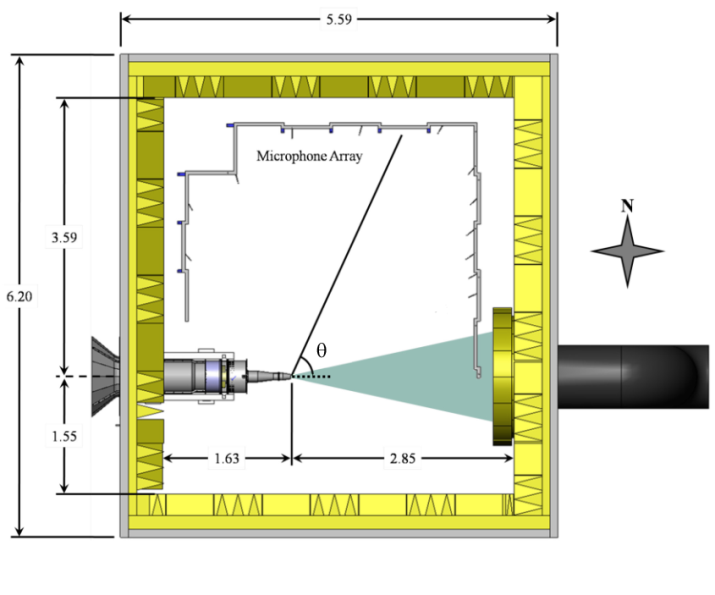
\includegraphics[width=3.5in]{GDTL_facility_schematic.png}
		\caption{Plan view of GDTL free jet facility and anechoic chamber; dimensions in meters.}\label{GDTLschematic}
	\end{center}
\end{figure}
	
Excitation was applied to jet shear layer via eight LAFPAs which were uniformly spaced around the nozzle perimeter 1 mm upstream of the nozzle exit. 
Each LAFPA consists of a pair of tungsten pin electrodes with tip spacing (center-to-center) of 4 mm. 
The electrodes are housed in a boron nitride extension attached to the end of the nozzle. A more detailed description of LAFPA characteristics can be found in Utkin et al. \cite{uyg2007-1}. 
The LAFPAs are energized by a multi-channel, high-voltage plasma power generator capable of simultaneously powering up to eight LAFPAs, which was designed and built in-house at the GDTL. 
In the second-generation power supply, each individual circuit consists of a switchable capacitor in line with a high voltage transformer; the arcing electrodes are connected to the secondary side of the coil. 
The switches are controlled by a 16-channel digital I/O card and National Instruments' Labview software, operated by a dedicated computer. 
The plasma generator provides independent control of the frequency, duty cycle/pulse width, and phase of each individual actuator (though at a constant amplitude of 5 kV). 
The pulse width was held constant at 7 $\mu$s, which was found to be the minimum pulse width at which the actuators consistently arced for all frequencies explored in this study \cite{hkfs-2011}. 

%%This got weird symbolly
%Near-field and far-field pressure measurements were acquired simultaneously, using Br\FCel \& Kj\E6r 1/4 inch 4939 microphones. The signal from each microphone is band-pass filtered from 20 Hz to 100 kHz using a Br\FCel \& Kj\E6r Nexus 2690 conditioning amplifier, and recorded using National Instruments PXI-6133 A/D boards and LabView software. 
Near-field and far-field pressure measurements were acquired simultaneously, using Bruel \& Kjear 1/4 inch 4939 microphones. 
The signal from each microphone is band-pass filtered from 20 Hz to 100 kHz using a Bruel \& Kjear Nexus 2690 conditioning amplifier, and recorded using National Instruments PXI-6133 A/D boards and LabView software.
The microphones are calibrated using a Bruel \& Kjear 114 dB, 1 kHz sine wave generator. 
The frequency response of the microphones is flat up to roughly 80 kHz, with the protective grid covers removed. 
Voltage signals are collected at 200 kHz with 81920 data points per block; sub-blocks of 8192 data points were used when calculating short-time power spectral densities, resulting in a frequency resolution of 24.4 Hz. 
Ten blocks were recorded for each case, resulting in four seconds of data. Analysis of the far-field acoustic spectra found this length to be sufficient for statistical convergence of the turbulence statistics.
\begin{figure}
	\begin{center}
		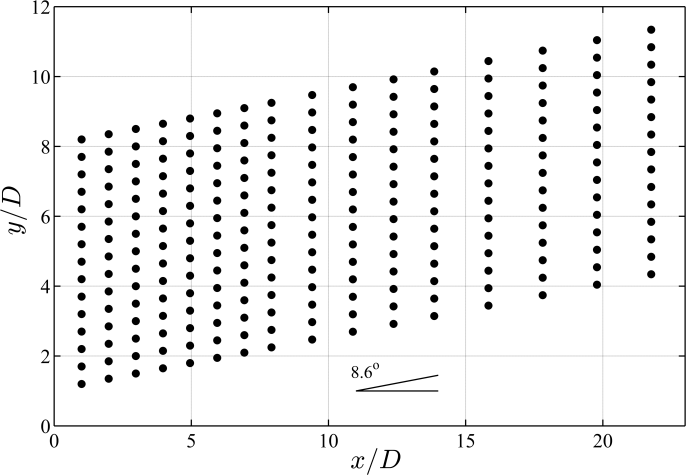
\includegraphics[width=3.5in]{GDTL_mic_locations.png}
		\caption{Near-field microphone array grid.}\label{mic_grid}
	\end{center}
\end{figure}

Far-field acoustic pressure is acquired at three polar angles: $30^{o}$, $60^{o}$ and $90^{o}$, as measured from the downstream jet axis. 
The radial distance of the microphones ranges from 101D at $30^{o}$ to 145D at $60^{o}$. 
The near-field pressure was acquired using a linear array of sixteen microphones located along the meridional plane of the jet; the spacing varied along the array from 1D to 2D (Fig. \ref{mic_grid}). 
The linear array is mounted to a traverse system at an angle of $8.6^{o}$ to the jet axis in order to match the spreading angle of the jet shear layer for this Mach number \cite{kfm2009-1}. 
The traverse is controlled using LabView and enables the acquisition of pressure measurements at various radial positions with respect to the jet axis. 
Initially, the most upstream microphone is positioned at x/D = 1 and r/D = 1.20, to ensure that the microphone tips are outside the mixing layer and do not affect the flow field. 
For subsequent cases, the microphone array is incremented radially outward by 0.5D for a total travel distance of 7D. 
Signals from the near-field array are preprocessed in order to remove actuator-self noise while retaining the true hydrodynamic and acoustic response of the jet. 
This has been accomplished via a filter operating in the continuous wavelet domain. Further details may be found in the work of Crawley \etal \cite{Crawley2015}.

\subsection{Computational Method}\label{theo}
The simulations employ the same approach as previously used
to successfully simulate Mach~$1.3$ and $0.9$ jets without and with
control\cite{gdv2011-POF,SpethCF2013,speth2014}.  The full compressible
Navier-Stokes equations are solved in curvilinear coordinates
($\xi,\eta,\zeta$) using the
strong conservative form\cite{vm74-1,sjl78-1}. The transformed
non-dimensional equations in 
vector notation are given as: 
\begin{equation}
\frac{\partial}{\partial\tau}\left(\frac{\vec{U}}{J}\right)+\frac{\partial\hat{F}}{\partial\xi}+\frac{\partial\hat{G}}{\partial\eta}+\frac{\partial\hat{H}}{\partial\zeta}=\frac{1}{Re}\left[\frac{\partial\hat{F}_{v}}{\partial\xi}+\frac{\partial\hat{G}_{v}}{\partial\eta}+\frac{\partial\hat{H}_{v}}{\partial\zeta}\right]\label{navier}
\end{equation}
where $\vec{U}=\left\{ \rho,\rho u,\rho v,\rho w,\rho E\right\} $
denotes the solution vector and
$J=\partial\left(\xi,\eta,\zeta,\tau\right)/\partial\left(x,y,z,t\right)$
is the transformation Jacobian.  Details of the various terms in
Eqn.~\ref{navier} may be found in Speth and 
Gaitonde\cite{speth2012b}.
For the inviscid terms, a third-order upwind biased approach is
adopted, together with the Roe scheme\cite{rpl81-1} for flux evaluation.  The
limiter required to enforce monotonicity is a crucial 
component of the method.  The van Leer harmonic limiter\cite{lbv79-1}
has proven to be very successful at reproducing the main features of the
unsteadiness in the jet.  The viscous 
terms are discretized with second-order centered differences and time
integration is performed by a second-order diagonalized~\cite{pth81-1}
approximately 
factored method~\cite{br78-1}.  A sub-iteration
strategy is used to minimize errors due to factorization, linearization and
explicit boundary condition implementation.
\begin{figure}
\begin{center}
	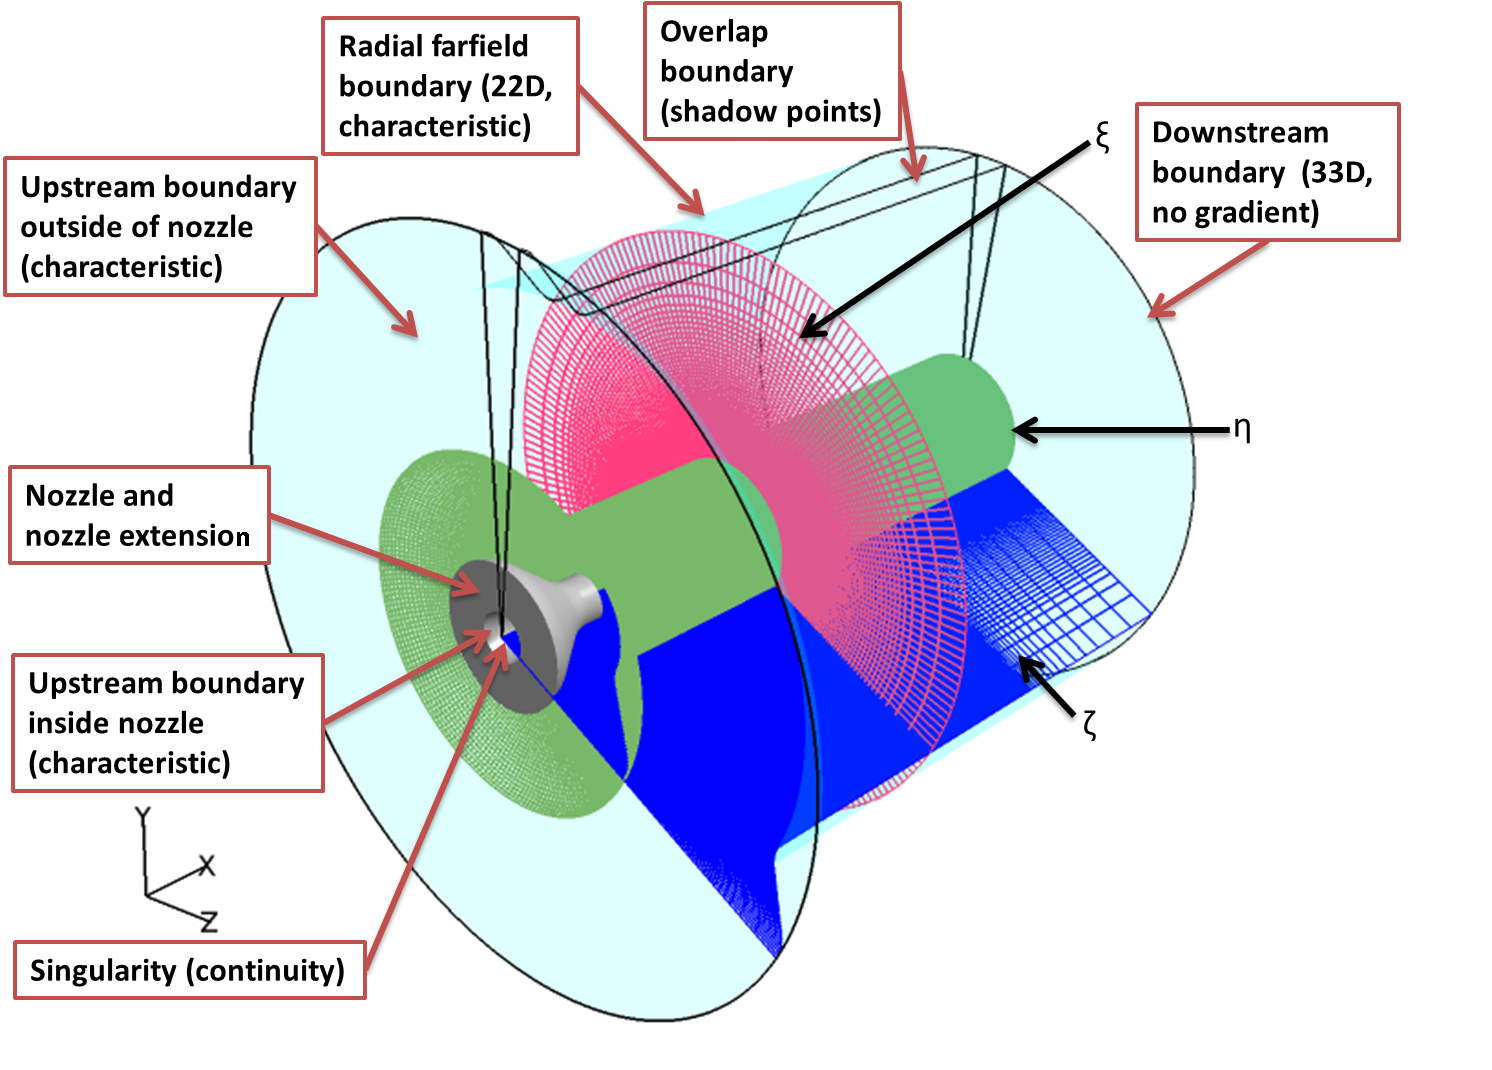
\includegraphics[width=3.5in]{MACH09ComputationalDomain1.png}
\caption{Computational domain}\label{fig:M09Computationaldomain}
\end{center}
 \end{figure}

 A $65$ million point mesh (Fig.~\ref{fig:M09Computationaldomain}) is
 used to simulate the Mach~$0.9$ jet measured in the experiment (Fig.
 \ref{GDTLschematic}).  The grid has dimensions of $685$ points on the
 $\xi$ (streamwise) direction, $455$ points in the $\eta$ (radial)
 direction, and $209$ points in the $\zeta$ (azimuthal) direction. In
 the radial direction, the mesh is refined in the nozzle region and
 gradually stretched in the far field. At the exit of the nozzle, the
 grid maintains a constant axial spacing until after the potential
 core length; then stretches in the streamwise direction. To
 preserve continuity, the grid has a five point overlap in the $\zeta$
 direction. Characteristic boundary conditions\cite{bj2000-1} are
 applied to the upstream (outside the nozzle) and radial boundaries.
 Non-reflecting conditions are applied to the downstream and far-field
 boundaries. Stagnation conditions are specified at the first $\xi$
 plane of the nozzle ($\rho_{inlet}=2.04kg/m^{3}$, $U_{inlet}=22m/s$, $P_{inlet}=171,427Pa$) to
 achieve perfectly expanded nozzle exit conditions corresponding to
 $\rho_{jet}=1.404kg/m^{3}$, $U_{jet}=285.99m/s$, $T_{jet}=251.31K$ which are similar to the experiments.
 Based on the nozzle diameter therefore, the Reynolds number is
 $Re=635,308$. The nozzle geometry resembles that of the 
 experiments including the nozzle ring on which the actuators are
 mounted. 
 The velocity profile at the entrance to the nozzle is that
 of a uniform flow (zero at the wall and $U_{inlet}$ everywhere else).
 Perturbations were not introduced into the inflow due to the
 unknown perturbations in the experiment. Therefore, the simulations
 have a laminar boundary layer at the nozzle exit while the
 experiments have a very thin turbulent boundary layer (the momentum
 thickness has been estimated to be $0.09 mm$).  Previous studies have
 shown that despite this difference, the main features of the
 experimental observations are successfully reproduced by the
 computations by a fixed longitudinal coordinate shift to account
 for the difference in the inlet characteristics of the experiment and computation\cite{gdv2011-POF,SpethCF2013}.  Other studies have shown
 that a smaller $32$ million point simulation is adequate to reproduce
 the features of the experiment\cite{spethASME2013}.

\begin{figure}[h]
\begin{center}
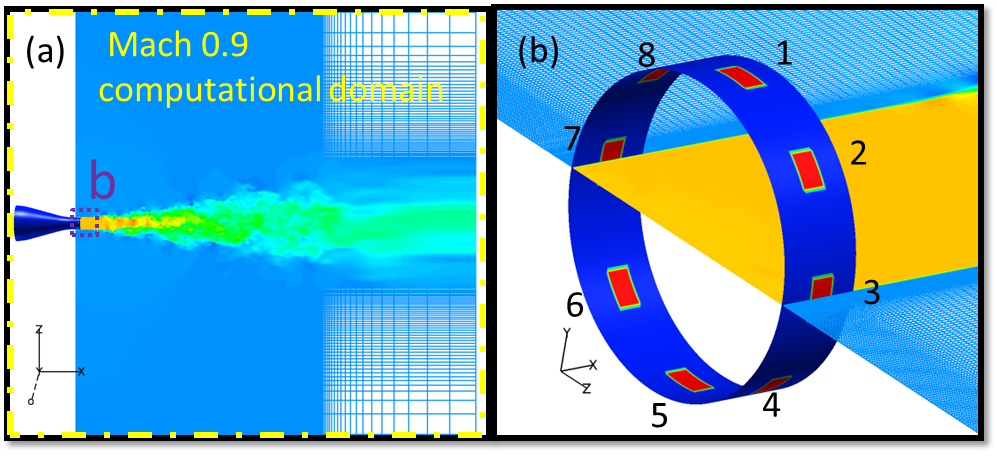
\includegraphics[width=3.6in]{actuatormodelnew}
\caption{The computational domain including the nozzle  (a), and the numerical actuator model (b)}\label{fig:actuator}
\end{center}
\end{figure}
The LAFPAs are modeled after the experiments using a surface heating
technique to excite jet shear layer instabilities and azimuthal modes
within the jet.  Eight actuators are placed around the periphery of
the jet on the nozzle collar at the locations and dimensions of the
experiments as explained previously. As shown in
Fig.~\ref{fig:actuator}b, each actuator consists of a heated region of
the nozzle wall which extends the azimuthal length corresponding to
the separation distance between electrodes ($3 mm$) and has an axial
extent equal to the length of the groove ($1 mm$). The temperature of
the nozzle wall was assumed to be $1.12T_{\infty}$.  When the actuator
is on the temperature of the actuator region increases to
$5T_{\infty}$. Little difference was seen in the previous work (Speth
and Gaitonde\cite{SpethASM2012}) for the temperature range measured in
experiments (Utkin {\em et al.}\cite{uyg2007-2}) for a Mach number of
1.3.  The semi-empirical model is necessary to avoid first-principles
simulation of the poorly understood plasma heating process, as well as
to restrict the required computational resources to feasible levels
(see Ref.~\citen{GaitondeCAF2013-1}).

Unlike acoustic drivers, the LAFPAs are on-off devices and thus can be
represented by rectangular pulses with a duty cycle, which allows for
a wide range of operation choices.  Duty cycle is the percentage of
actuator on time in an excitation cycle. Therefore, a duty cycle
of $100\%$ results in the actuator being on all the time.  
The experimental duty cycle varies with frequency, since the arc
strike lasts a fixed time.  Since the actuator
model is empirical, the computational duty cycle was chosen to obtain
similar control authority as in the experiment.  This necessitates a
higher
duty cycle ($10\%$) than the one used in the experiments
($2.0\%$ for $St_{DF}=0.25$).
As noted earlier, despite the simplicity of the model, its success
has been documented in Gaitonde 
and Samimy\cite{gdv2011-POF}, where, in addition to coherent
structures, mean and fluctuating quantities have been compared.
Furthermore, the mean flow structure with control was shown to match
the theoretical predictions of Cohen and Wygnanski~\cite{cj87-2}.

Due to the required amount of computational time, the number of excitation Strouhal numbers was reduced from the experimental set to a select number of interesting cases.
The Strouhal numbers studied in the
simulations include: $0.05$, $0.15$, and $0.25$. Data was acquired
every timestep at the point probes depicted in Fig.~\ref{mic_grid}
as well as on several $\xi$, $\eta$, and $\zeta$ computational planes.
Phase-averaged data were also computed for each of the simulations.

%%%%%%%%%%%%%%%%%%%%%%%%%%%%%%%%%%%%%%%%
\subsubsection{Grid Resolution Study}
 The variations due to grid resolution are depicted in Figures \ref{meangridM09} and \ref{meangridrmsM09} for both Mach numbers. Figure \ref{meangridM09} depicts the mean axial velocity along the centerline. Figure \ref{meangridM09} compares the three grids for the Mach 0.9 case with axisymmetric excitation. The three grids, are relatively similar although G1 has a slightly higher decay rate after the potential core. However, grids G2 and G3 exhibit the same decay rate after the potential core for the extent plotted. 
\begin{figure}
\begin{center}
{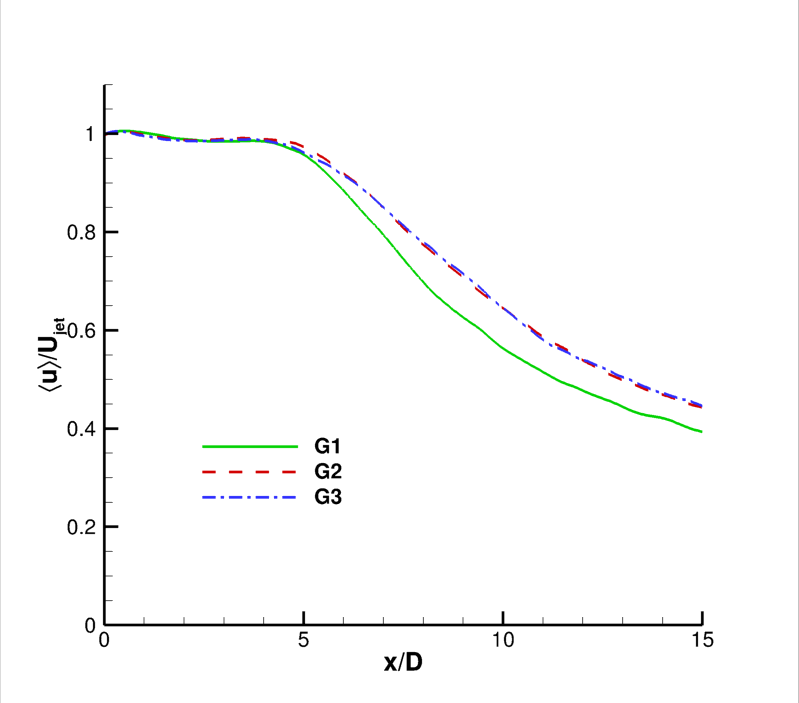
\includegraphics[width=3.2in]{gridstudyM09meancenter.png}\label{meangridM09}}
\caption{Grid convergence of the mean axial velocity along the centerline of the Mach 0.9, $m=0$, $St=0.15$ case}
\end{center}
 \end{figure}

Figure \ref{meangridrmsM09} depicts the root-mean-square (RMS) fluctuating axial velocity along the centerline of the jet. The relative shape and amplitude of the fluctuating velocities is the same for each grid. Therefore, there is a very small
effect in terms of the principal coherent features and jet core
length, but modest sensitivity was evident. This is to be expected in implicit large eddy simulation in which no subgrid model is used. Due to the concern of nearfield wave propogation grid G3 will be used. 
\begin{figure}
\begin{center}
{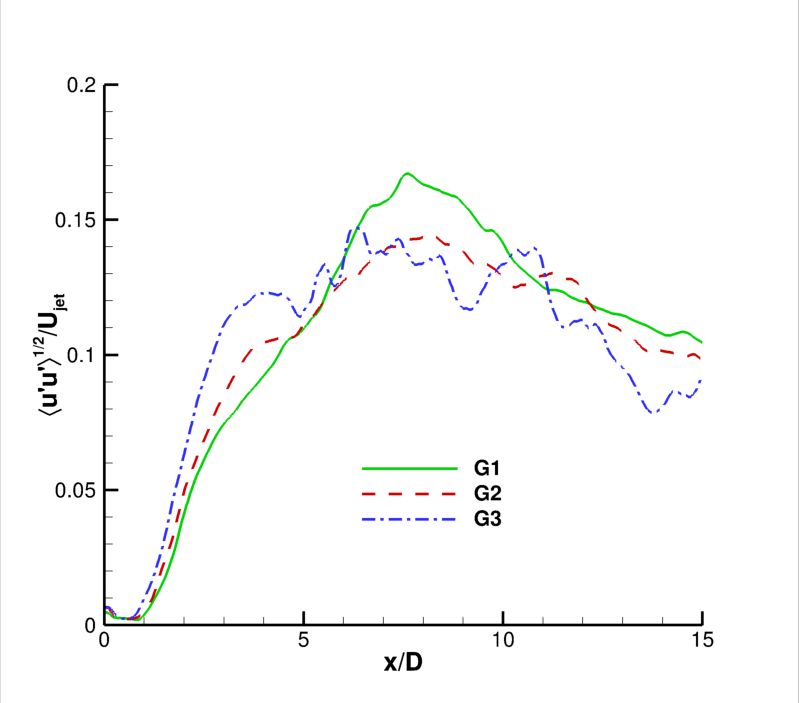
\includegraphics[width=3.2in]{gridstudyM09rmscenter.png}
\label{meangridrmsM09}}
\caption{Grid convergence of the RMS fluctuating axial velocity along the centerline of the Mach 0.9, $m=0$ $St=0.15$ case}
\end{center}
 \end{figure}

%%%%%%%%%%%%%%%%%%%%%%%%%%%%%%%%%%%%%%%%%%%%%%%%%%%%%%%%%%%%%%%%%%%%%%%%%%%%%%%%%%%%%%%%%%
\subsubsection{Numerical Validation}
To begin, the computations will be compared to experimental results of Crawley {\em et al.} \cite{Crawley2014}. These comparisons will prove not only that the schemes used for the LESs capture the physics of the flow but also the actuator model is able to produce structures similar to the experiments.

The axial decay of the streamwise velocity along the centerline for the no-control case is depicted in Fig. \ref{umeanexpcompNC}. The simulation data was shifted to account for the unknown turbulence in the experimental nozzle boundary layer. 
The boundary layer of the experiments is known to be thin and turbulent \cite{kastnerj2009-1}. These simulations however have a uniform flow field applied to the first axial plane. This allows for a natural laminar boundary layer to form due to the computation of the whole nozzle. The effect of the boundary layer thickness is discussed by Speth and Gaitonde \ref{Speth2014}. The perturbations within the nozzle affect the dynamics of the jet as shown by Bogey {\em et al}. \cite{bogey2012}. 
For simplicity and grid conservation, perturbations are not employed in the nozzle/nozzle ring. Therefore, the  un-controlled jet was shifted $1.4D$.  The decay rate after the potential core are similar and match the experimental results well.
\begin{figure}
\begin{center}
\subfloat[Mean centerline axial velocity]{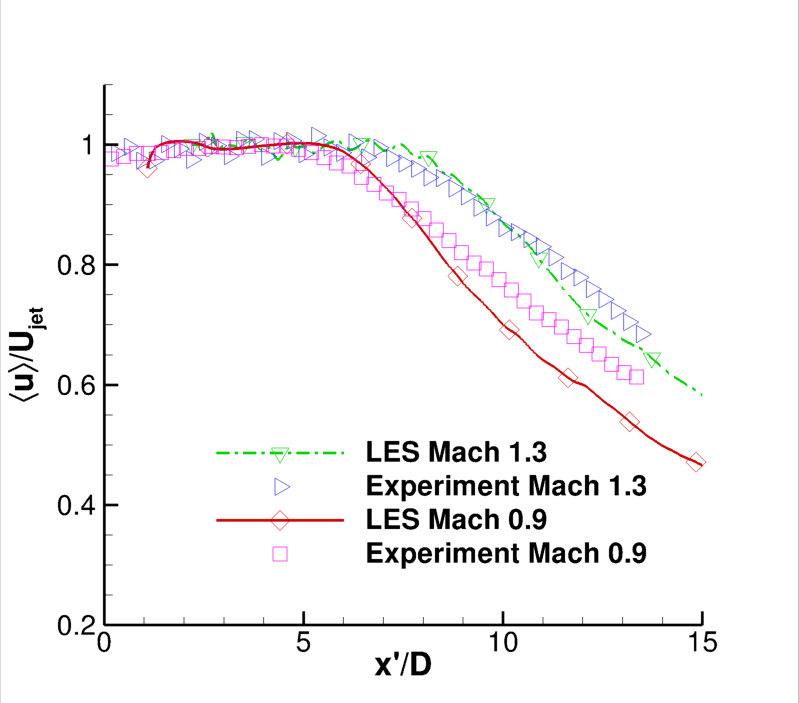
\includegraphics[width=3.2in]{expcompmeancenterM0913NC}
\label{umeanexpcompNC}}
\subfloat[Centerline axial RMS fluctuations]{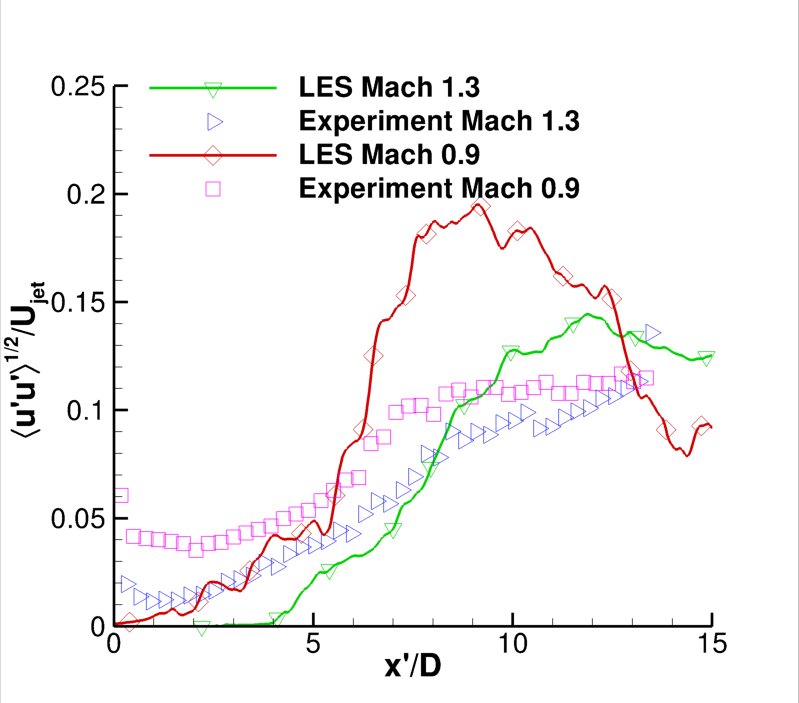
\includegraphics[width=3.2in]{expcompupcenterM0913NC}
\label{upexpcompNC}}
\label{expcompNC}
\caption{Non-dimensional mean and RMS centerline velocities for the uncontrolled jets}
\end{center}
 \end{figure}

Figure \ref{upexpcompNC} exhibits the growth of the axial root mean square (RMS) fluctuations on the centerline for the no-control case with experimental results. The simulation is shifted the same distance as in Fig. \ref{umeanexpcompNC}. Since no turbulence is added to the simulations within the nozzle/nozzle ring, the fluctuations start at zero (unlike the experiment). The Mach $0.9$ jet has a maximum RMS value around $x/D=8$ which corresponds to downstream of the potential core ($x/D=6$). The supersonic jet peaks after the potential core ($x/D=7.5$) at an axial distance of 12D. 

Figure \ref{expcompST025} shows the centerline axial mean and fluctuating velocity for the $St=0.25$ excitation cases with experimental results by Samimy {\em et al.} \cite{sm2007-2,kearney2013intermittent}. Note that, the experimental Mach $0.9$ centerline results have an excitation frequency of $St=0.35$ while the simulation data and the experimental irrotational pressure data for this Mach number have an excitation frequency of $St=0.25$. The simulation data for Figs. \ref{expcompST025}a and b were shifted axially by $0.84D$ for the $M=0.9$ case to match the core length. The decay rate of the centerline axial velocity for the simulations matches the experimental rates similar to the no-control results.  Figure \ref{upexpcompST025} depicts the axial RMS fluctuations along the centerline for the excited case. The simulation has similar growth to the experimental results throughout the potential core. After the potential core the simulation consistently over predicts the experimental results.
\begin{figure}
\begin{center}
\subfloat[Mean centerline axial velocity]{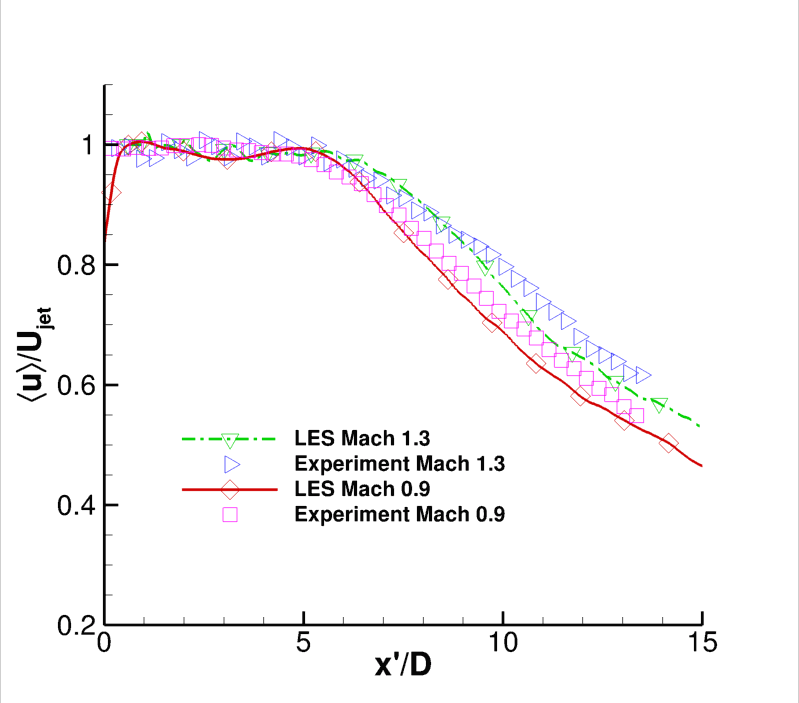
\includegraphics[width=3.2in]{expcompumeancenterM0913}
\label{umeanexpcompST025}}
\subfloat[Centerline axial RMS fluctuations]{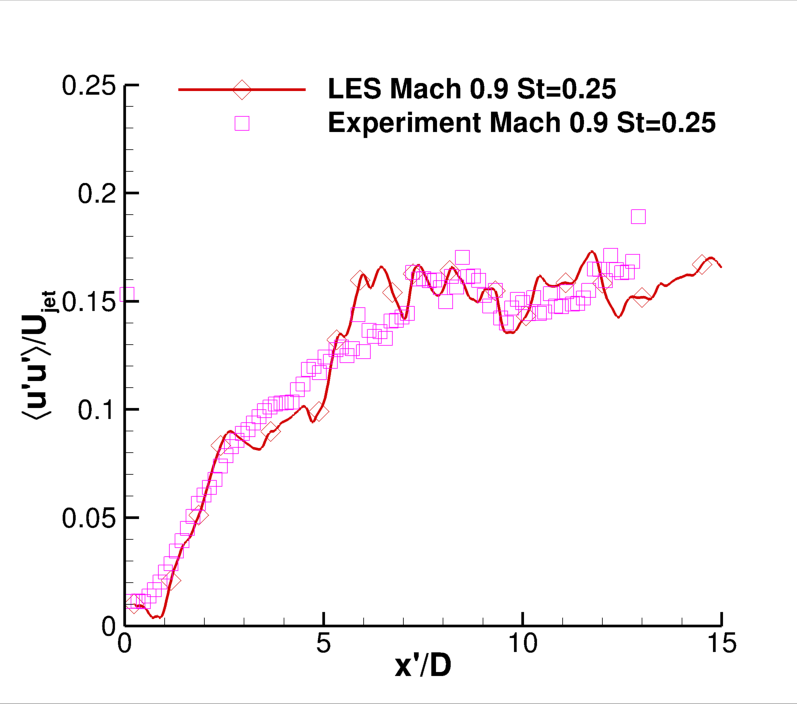
\includegraphics[width=3.2in]{expcompupcenterM0913}
\label{upexpcompST025}}
\label{expcompST025}
\caption{Non-dimensional mean and RMS centerline velocities for the jets controlled with the axisymmetric mode at a $St=0.25$ }
\end{center}
 \end{figure}


When the jet is excited with the plasma actuators using specific modes large scale structures develop in the shear layer and propagate downstream. For the axisymmetric mode, ring structures form that show up as vertically aligned vortices in cross-sectional slices as shown in Fig. \ref{galilcomp}. Figure \ref{galilcomp} depicts the phase-averaged contours of Galilean streamlines with the background colored by axial velocity for both the experiments and the computations. Galilean streamlines are formed by subtracting the convective velocity ($U_{convect}=0.65U_{jet}$) from the velocity field of the instantaneous or in this case phase-averaged snapshot. The simulations were shifted to match the potential core length of the experiments due to the unknown boundary layer properties at the exit of the nozzle extension. The effect of the boundary layer thickness and turbulence level is discussed further in Section \ref{thicknesseffects}. In Fig. \ref{galilcomp}, both experiments and computations have 3 distinct vortical rings before the end of the potential core.  Therefore, although the initial turbulence level of the boundary layer is not captured the large scale dynamics remains similar. 
\begin{figure}
\begin{center}
\subfloat[Experiment]{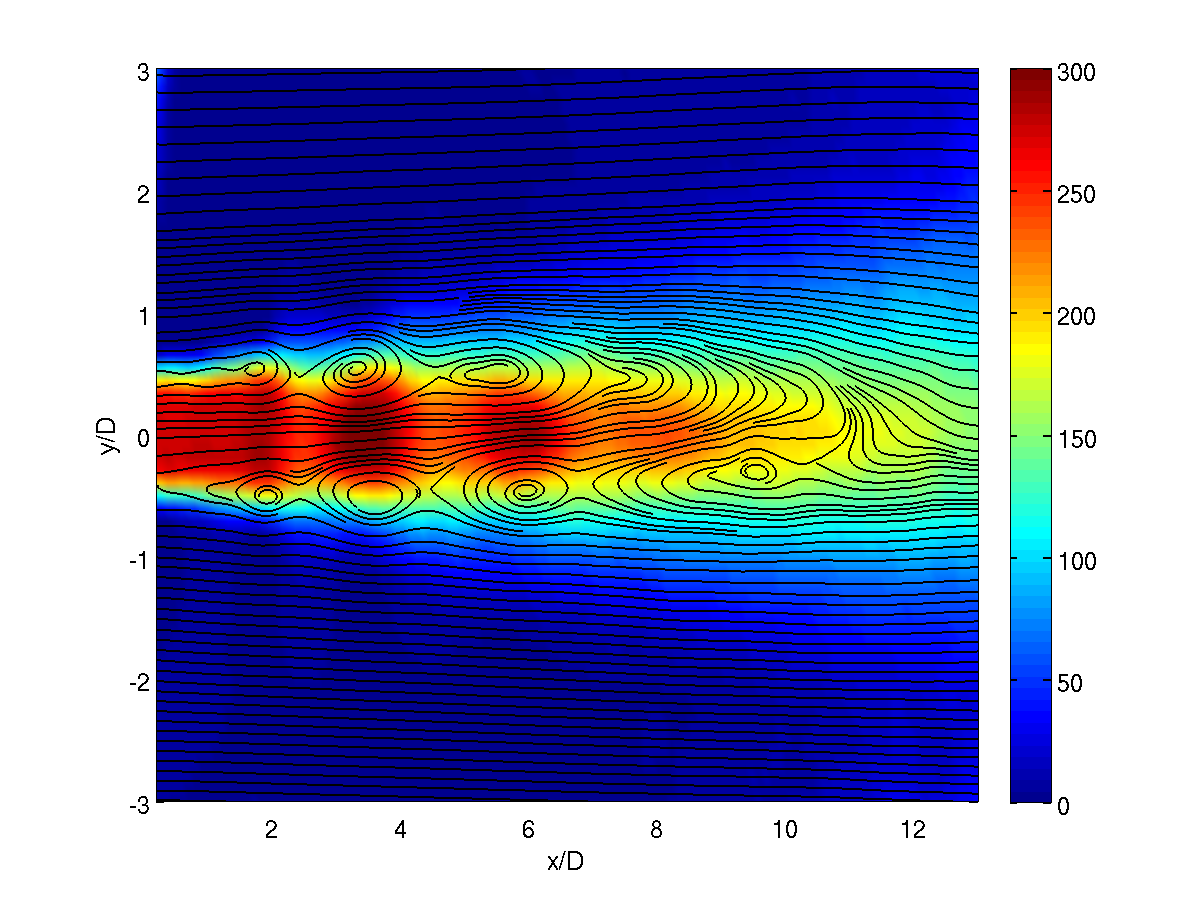
\includegraphics[width=3.2in]{galileanm0ST025expM09.png}
	\label{galilexp}}
\subfloat[Simulation]{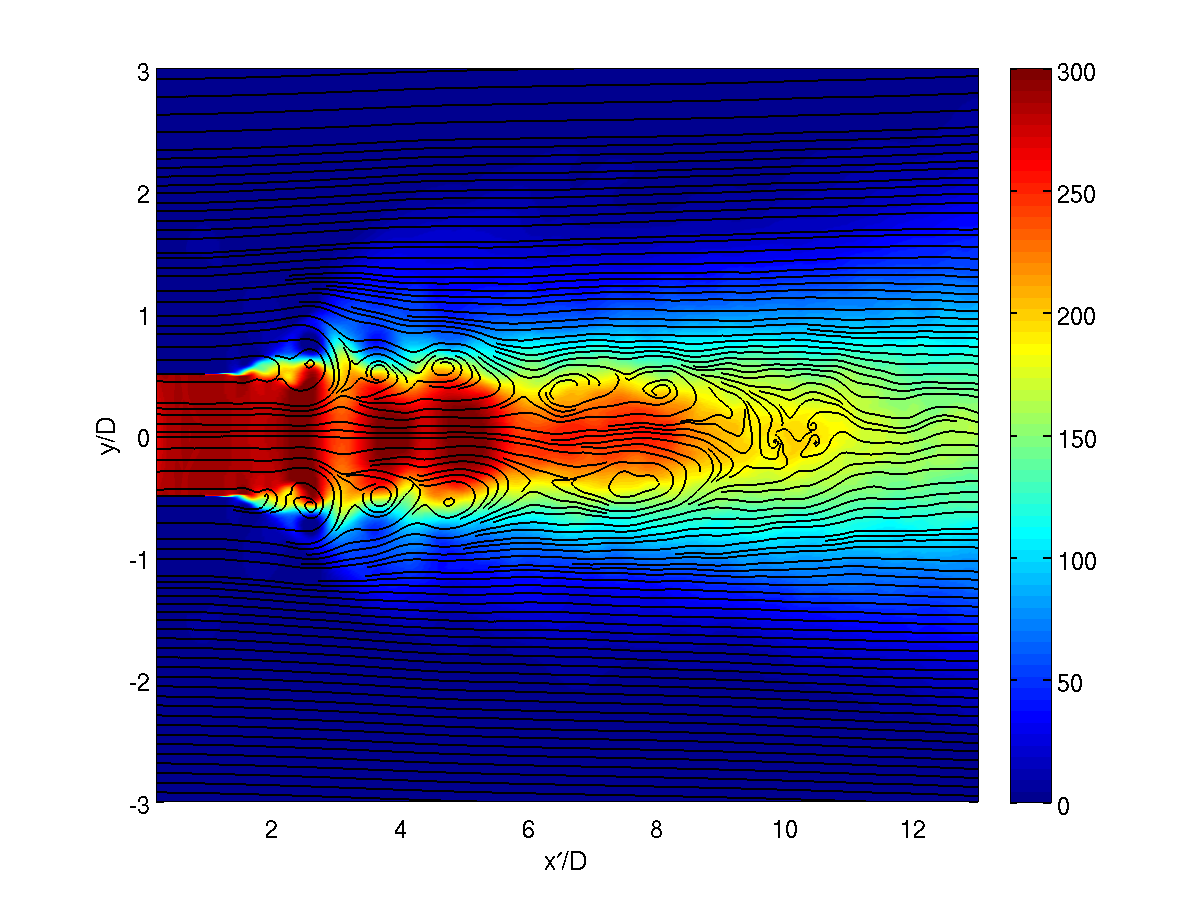
\includegraphics[width=3.2in]{galileanxshift06St025M09}
\label{galilsim}}
\label{galilcomp}
\caption{Phase-averaged structures highlighted by Galilean streamlines for the axisymmetric mode at a $St=0.25$}
\end{center}
 \end{figure}

The coherent structures that develop in the jet (Fig. \ref{galilcomp}) affect the near field and thereby the sound generation. 
To understand the near field dynamics of the excited jets, point probe arrays were placed at radial locations corresponding to Fig. \ref{mic_grid}. 
Figure \ref{fig:pointprobeM09} depicts the gauge pressure of the $St=0.25$ forced Mach 0.9 simulation and experiment located at $x/D=2$ on $Array~1$. Also shown is the actuator temperature versus time. The simulation pressure was divided by a factor of $2.3$ in order to match the experimental wave amplitude. The amplitude of the pressure waves are highly dependent on pressure probe location accuracy, actuator location, nozzle lip width, and nozzle exit boundary layer conditions making it difficult to match quantitatively \cite{sinha2013}. Qualitatively, the experimental pressure depicts a sharp discontinuous region ($t=0.01113s$ and $0.01165s$)  before a pressure wave (extremas located at $t=0.01114s$ and $0.01118s$) consisting of a peak followed by a trough. The discontinuous region is associated with the actuator self-noise while the pressure wave is associated with the large scale structure generated by the actuator perturbation. The self-noise is a compression wave generated by the actuators that moves at the speed of sound and can be seen in the near field. In the simulation, the discontinuous region is not present. Instead, there is a small secondary peak in the upward rise of the pressure wave. Since the effect of the actuators is modeled rather the shock-like structure that occurs in the experiment is not captured. The effect of the actuators on the dynamics of the jet is captured however. 

To further convey that the dynamics of the jet are captured, Fig. \ref{fig:phasex2all} plots the phase-averaged waveforms for the experiment and simulation on $Array~1$ for a $St=0.25$. Observe that the effect of the actuator self-noise seen in the experimental data diminishes with axial distance. The hydrodynamic waves created by the excitation pulse form a sine-like pattern by $x/D=2$. These waves increase in amplitude from $x/D=1$ to $2$ (within the potential core). Far beyond the potential core, at $x/D=12$, the periodic waves have diminished in amplitude but maintain a sine-like structure. This reduction is due to the break up of the large scale structures created by the actuator pulse beyond the potential core. 
%%%%%%%%%%%%%%%%%CHECK PLOTSSSSSSSSSS????????????????????????????????????????????????????

\begin{figure}
\begin{center}
	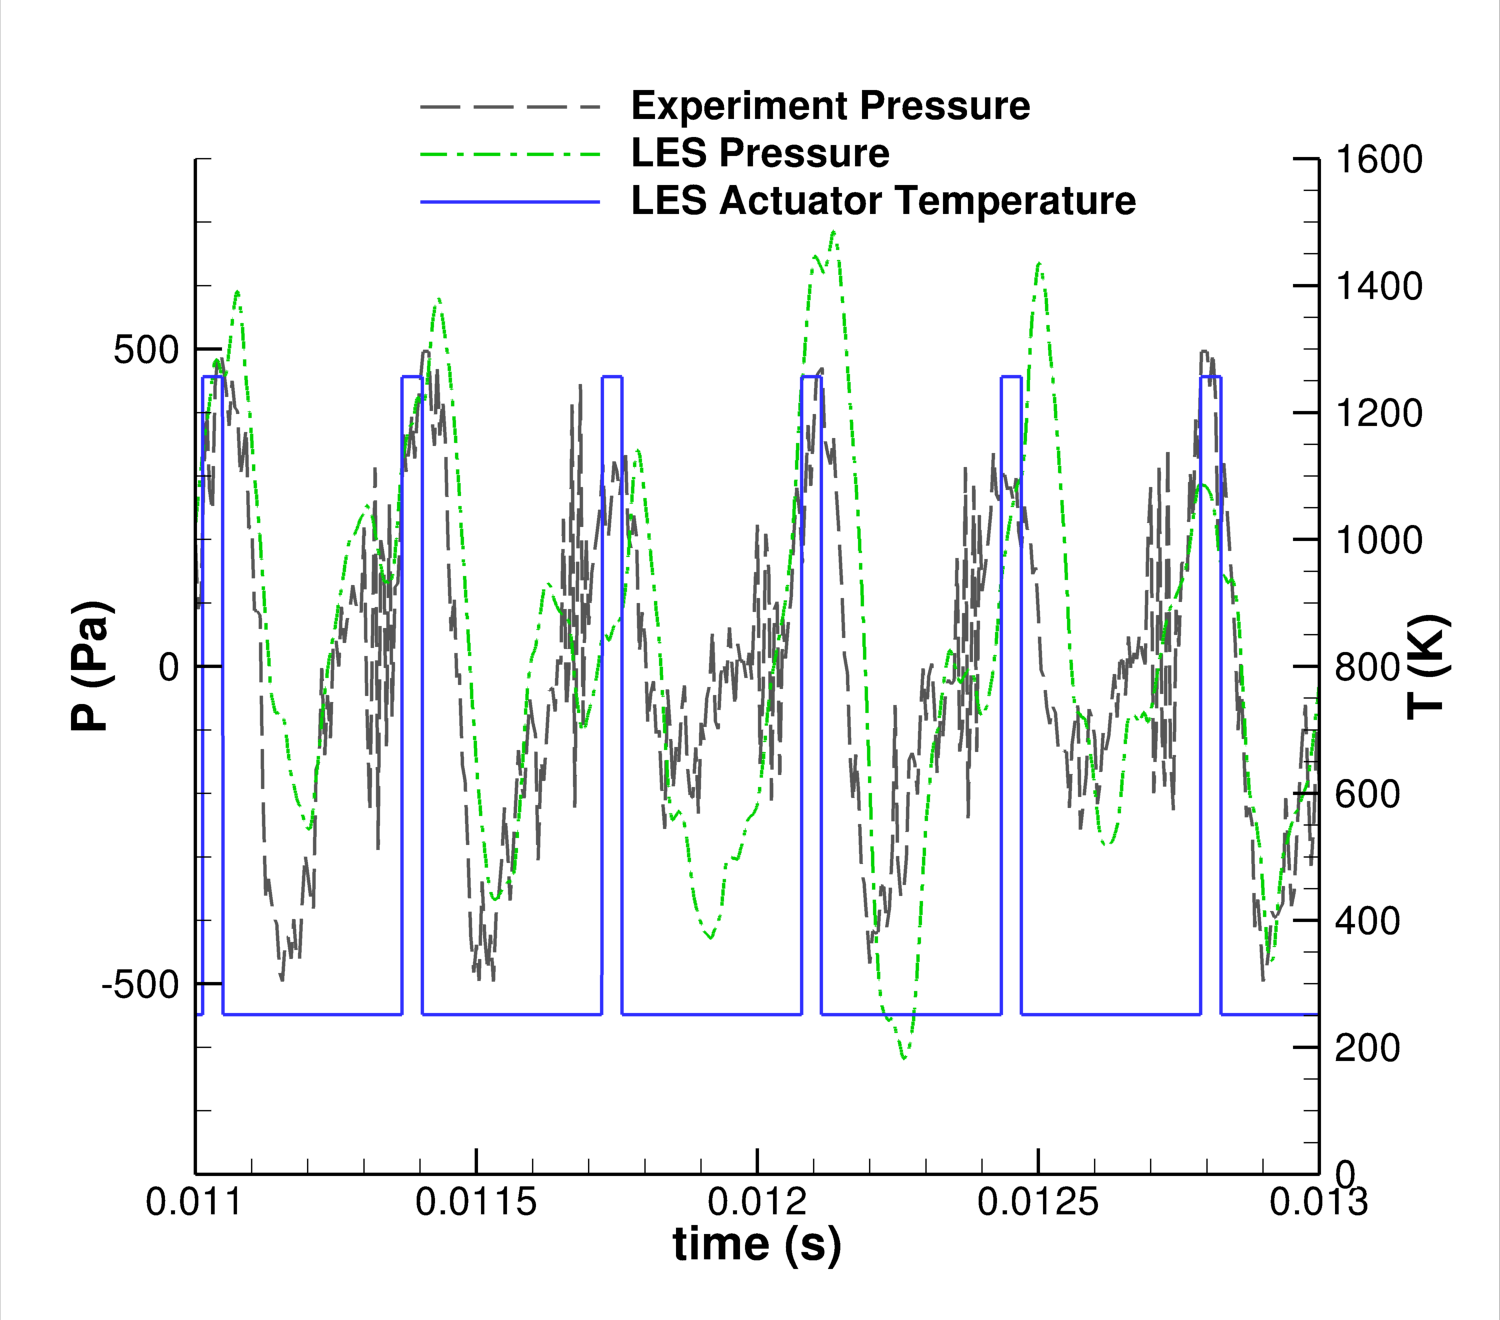
\includegraphics[width=3.5in]{M09pointwithactuatorx2array1ST025}%fixed
	\caption{Near field pressure response for the St=0.25 forced Mach $0.9$ jet and the actuator temperature at $x/D=2$ on $Array~1$ with experimental results \cite{Crawley2014}}
	\label{fig:pointprobeM09}
\end{center}
\end{figure}
\begin{figure}
\begin{center}
	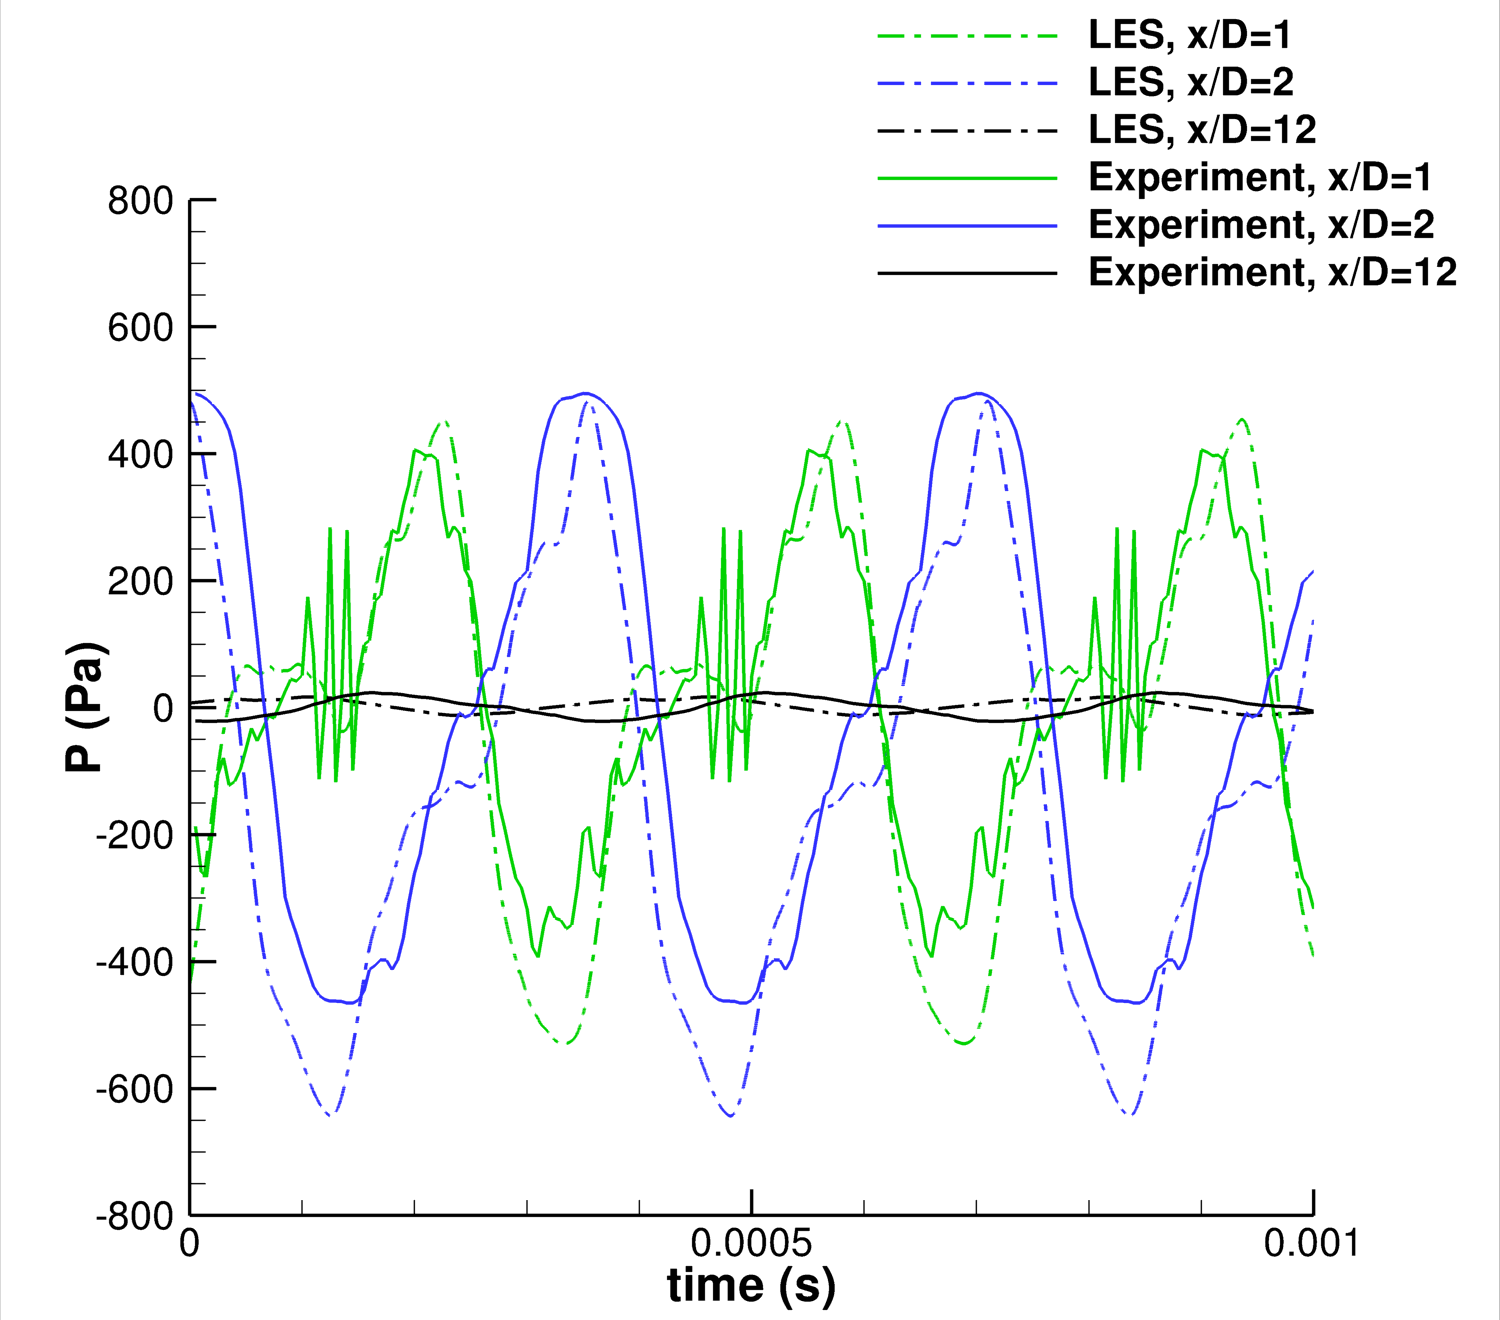
\includegraphics[width=3.5in]{M09LESandExpaxialphase}%fixed
\caption{Phase-averaged waveforms on $Array~1$ for experiment \cite{Crawley2014} and LES with St=0.25 excitation for Mach 0.9}
\label{fig:phasex2all}
\end{center}
 \end{figure}

%%%%%%%%%%%%%%%%%%%%%%%%%%%%%%%%%%%%%%%%%%%%%%%%%%%%%%%%%%%%%%%%%%%%%%%%%%%%%%%%%%%%%%%%%%%%%
\section{Results}\label{results} 
%%%%%%%%%%%%%%%%%%%%%%%%%%%%%%%%%%%%%%%%%%%%%%%%%%%%%%%%%%%%%%%%%%%%%%%%%%%%%%%%%%%%%%%%%%%%%
\subsection{Evolution of the Large-Scale Structures}\label{structure}
%%%%%%%%%%%%%%%%%%%%%%%%%%%%%%%%%%%%%%%%%%%%%%%%%%%%%%%%%%%%%%%%%%%%%%%%%%%%%%%%%%%%%%%
The majority of the sound heard in the downstream angles is due to the coherent structures developed in the shear layer. Therefore, to begin, the formation and decay of these structures will be analyzed. The phase-averaged isolevels of Q-criterion ($Q=0.35$) colored by axial velocity with a background of dilatation in gray scale are illustrated in Figs. \ref{fig:isolevels05} through \ref{fig:isolevels} for each excitation case. Each figure depicts two phases of the excitation period ($\phi =0.1(2\pi)$ and $0.6(2\pi)$). In each phase, the locations of $x/D=2$ and $4$ of $Array~1$ (array locations shown in Fig. \ref{mic_grid}) are labeled. 
For all cases, small individual vortical rings are produced near the
nozzle exit by the break down of the shear layer. As these vortical
rings move downstream they become bigger for the two higher
frequencies.  This is accompanied by the spreading of the jet due to
entrainment.  This is not readily seen in the phases depicted for the low frequency case due to the structure already having convected out of the viewing area. At the higher frequencies, streamwise ribs connecting
successive rings are also evident\cite{gdv2011-POF}: these represent
increasing interaction between successive rings.  These connect the
outer part of one ring to the inner part of the previously generated
structure, where the velocity is higher.  The subsequent decay of
the large structures is clearly evident.  At any given location, the
degree of prominence of the rollers depends on the phase: for example,
in the $St=0.15$ case, there is a well formed roller at about $x/D=4$ at
$0.1(2\pi)$ phase but at $0.6(2\pi)$ the roller is broken
down at the same axial location.  Similar effects can be seen in the
phase averaged results for the $St=0.25$ case. Another feature of the
flow is the presence of hair-pin like structures, which are especially
prominent in the higher frequency cases: note for example the
structure at $0.6(2\pi)$ for $St=0.25$ slightly before the $x/D=2$
probe.
For the $St=0.05$ cases (Fig. \ref{fig:isolevels05}), the A' and A structures are depicted in the phase $0.1(2\pi)$. At the phase of $0.6(2\pi)$, the structure in the first phase has already broken up resulting in no observable actuator induced structures in this phase. 
\begin{figure}
\begin{center}
\begin{centering}
{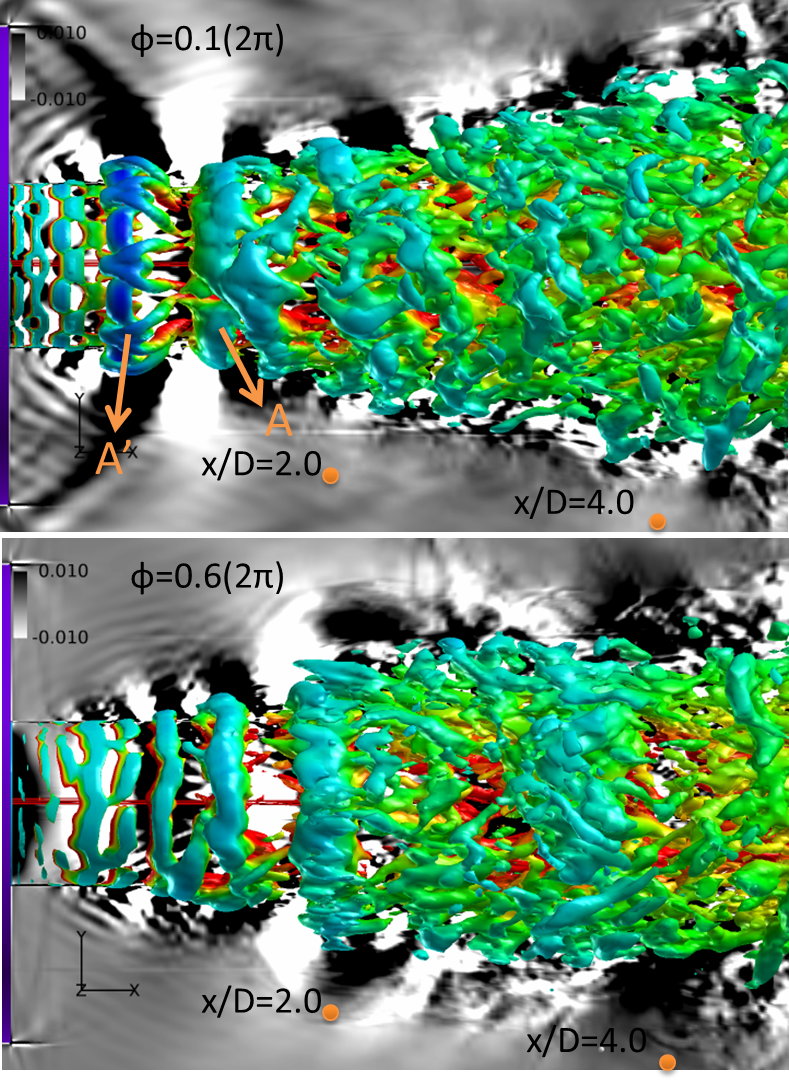
\includegraphics[width=2.6in]{M09St005qcritphase0106AB}}
\end{centering}
\caption{Iso-levels of Q-criterion colored by axial velocity with dilatation in gray scale for the St=0.05 cases}
\label{fig:isolevels05}
\end{center}
\end{figure}

For the high frequency cases, rollers develop due to the excitation and these rollers grow and interact with other actuator induced structures as they propagate downstream. This has been shown experimentally by Sinha \etal \cite{sinha2013}. The structures that are produced in phase $\phi=0.6(2\pi)$ of Figs. \ref{fig:isolevels15} and \ref{fig:isolevels} are the same as the impulse response structures in Fig. \ref{fig:isolevels05} but as the structures grow and propagate downstream they interact with the previously created actuated structure. The structures seen in Fig. \ref{fig:isolevels05} are labeled in Figs. \ref{fig:isolevels15} and \ref{fig:isolevels} for comparison. Structures B and B' are equivalent to A and A' respectively and belong to the previous/subsequent actuator pulse. 
Figure \ref{fig:isolevels15} depicts the $St=0.15$ cases in which the structures start to interact around an axial distance of 4D. In phase $\phi=0.1(2\pi)$, the characteristic structures seen in Fig. \ref{fig:isolevels05} are seen. Half a phase later A' is broken up close to $x/D=4$ while the ill formed B structure is colliding into the remains of A'. B' and B are similar structures to the ones denoted in the impulse case (Fig. \ref{fig:isolevels05}) however structure B is not as well formed as structure A. While, B' is more robust than the previous A' structure. This indicates a degree of feedback response of the structures between each excitation pair. %%%%%%%DOES IT?? HOW DO I CHECK????
% % % % % %[I'm not sure you can check this in the phase-averaged results. My inclination would be to look at the time-resolved data] - MC
\begin{figure}
\begin{center}
\begin{centering}
{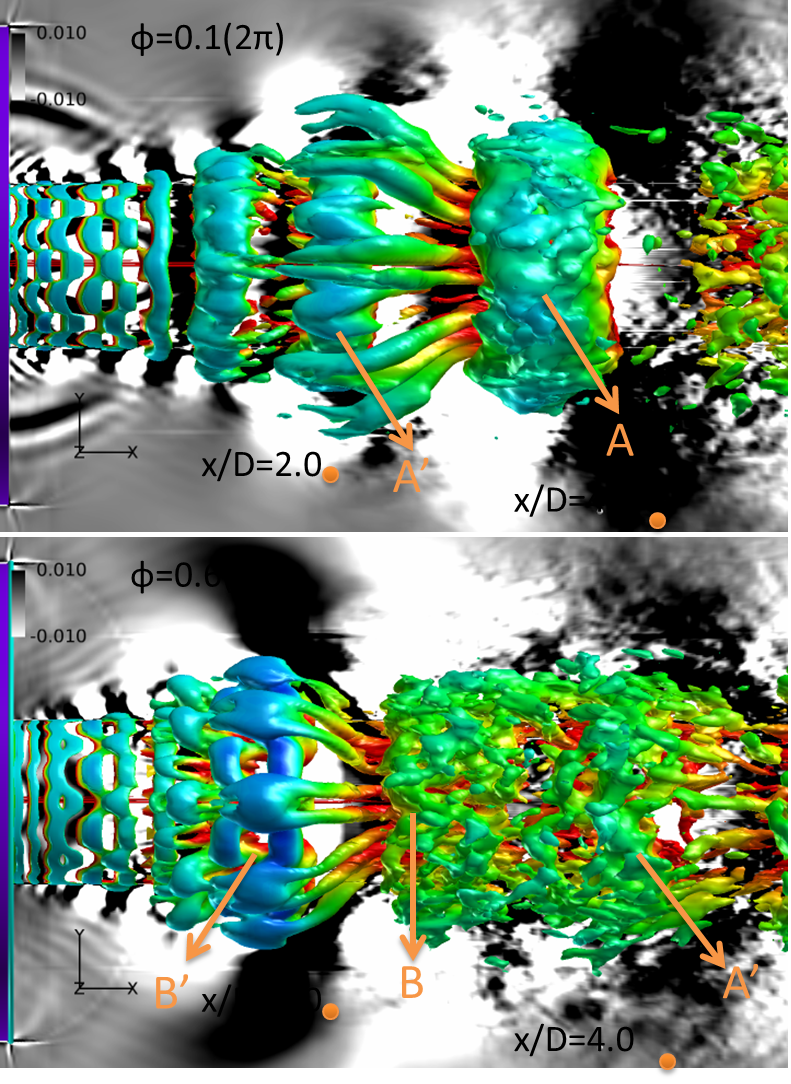
\includegraphics[width=2.6in]{M09St015qcritphase0106AB}}
\end{centering}
\caption{Iso-levels of Q-criterion colored by axial velocity with dilatation in gray scale for the St=0.15 cases}
\label{fig:isolevels15}
\end{center}
\end{figure}

Figure \ref{fig:isolevels} depicts the isolevels of the high frequency ($St=0.25$) case in which the structures are interacting by an axial distance of $2D$.
Since, the reaction to the actuation is cyclic the structures seen at the end of the potential core in one phase ($\phi=0.1(2\pi)$) begin to develop in the other phase. Structure B/A' in phase $\phi=0.1(2\pi)$ occurs when structure B collides into structure A'. This compression occurs due to the high convective velocity of B compared to A'. This interaction is quasi-linear creating a sine-like response in the near field pressure through linear superpositioning of the two actuator structures (B and A'). This quasi-linear superpositioning was also seen in Sinha \etal \cite{sinha2013} and Crawley \etal \cite{Crawley2014}. This will be discussed further later in reference to Fig. \ref{NUM_Phase_AVG_lip}.
\begin{figure}
\begin{center}
\begin{centering}
{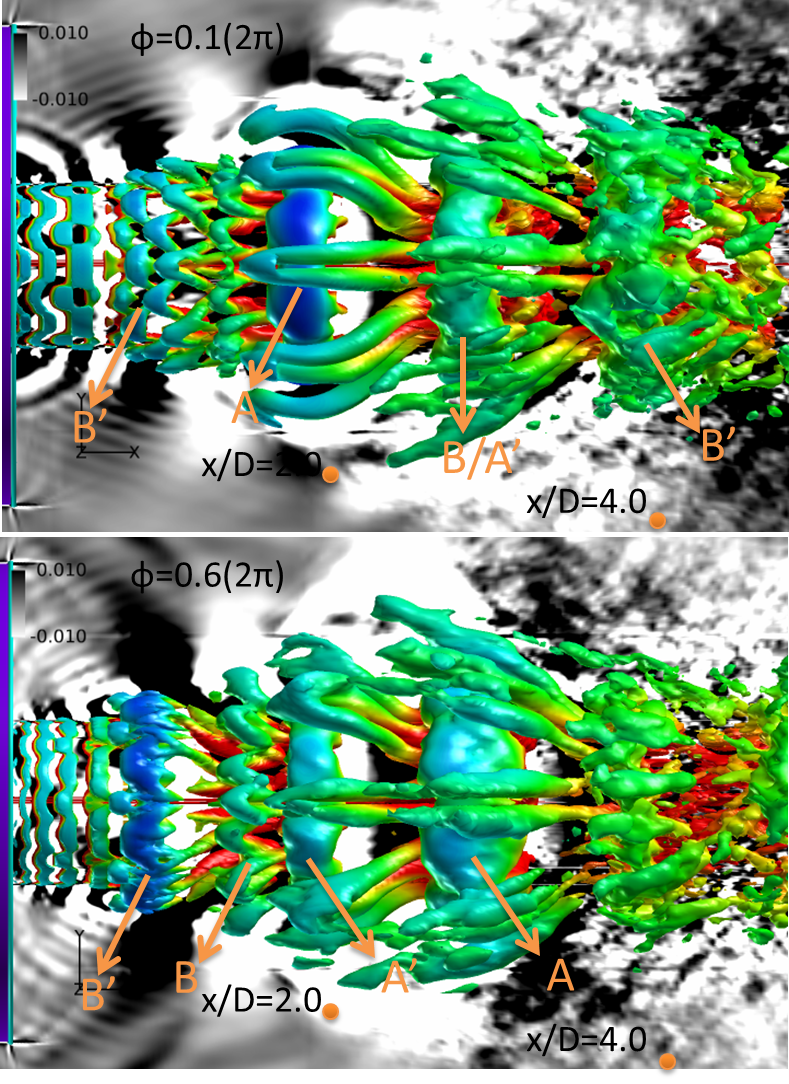
\includegraphics[width=2.6in]{M09St025qcritphase0106AB}}
\end{centering}
\caption{Iso-levels of Q-criterion colored by axial velocity with dilatation in gray scale for the St=0.25 cases}
\label{fig:isolevels}
\end{center}
\end{figure}

%The effect of the hairpin structures can be further envisioned by Fig. \ref{CSvr} which shows the phase-averaged radial velocity normalized by the jet velocity on an axial cross-section of the jet for the first well developed roller located around x/D=2 for an excitation of St=0.25 along with a lower duty cycle for the for comparison. The jet has higher outward velocity regions in-line with the placement of the eight actuators which corresponds to the hairpin vorticies in Fig. \ref{fig:isolevels}a and entrainment of the high speed core flow into the coherent structures. In between the hairpin vortices there is indication of the ambient fluid being entrained into the coherent structure ring due to the negative radial velocity. The low duty cycle case exhibits this same process but the legs of the hairpins do not extend as deep into the core. However, the hairpins of both subsonic duty cycle cases have similar strengths at this axial location. The similarity between the two duty cycles conforms with the findings of Speth and Gaitonde \ref{SpethCF2013} in which the duty cycle had little effect on a Mach 1.3 perfectly expanded jet.
 
%%%%%%%%%%%%%%%%%%%%%%%%%%????IS THIS DUE TO DUTY OR THE COMPRESSIBILITY???????????
%\begin{figure} 
%\begin{centering}
%\subfloat[St=0.25, 10\% duty cycle]{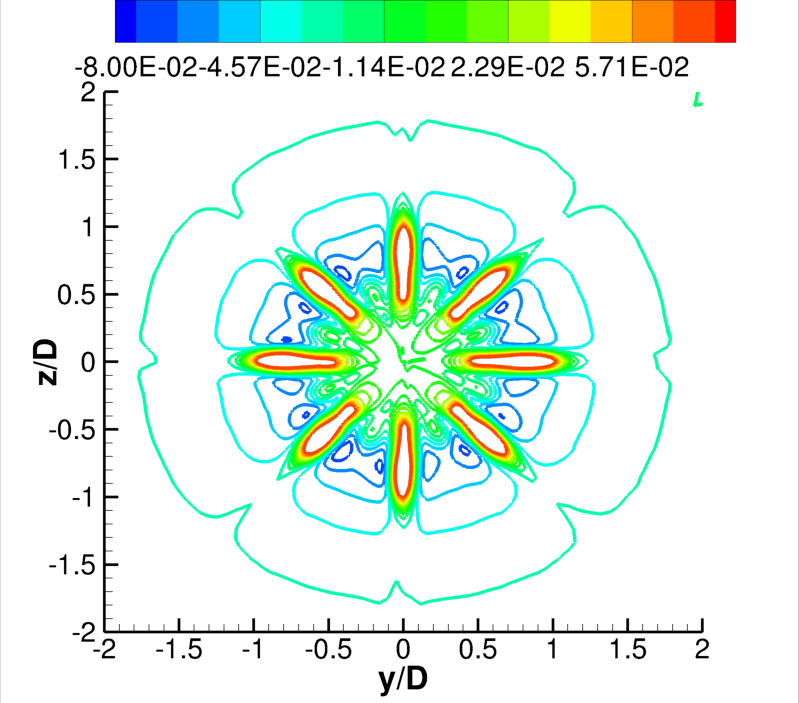
\includegraphics[width=3in]{M09ST025x2vraxialcross}} %fixed
%\subfloat[St=0.25, 3\% duty cycle]{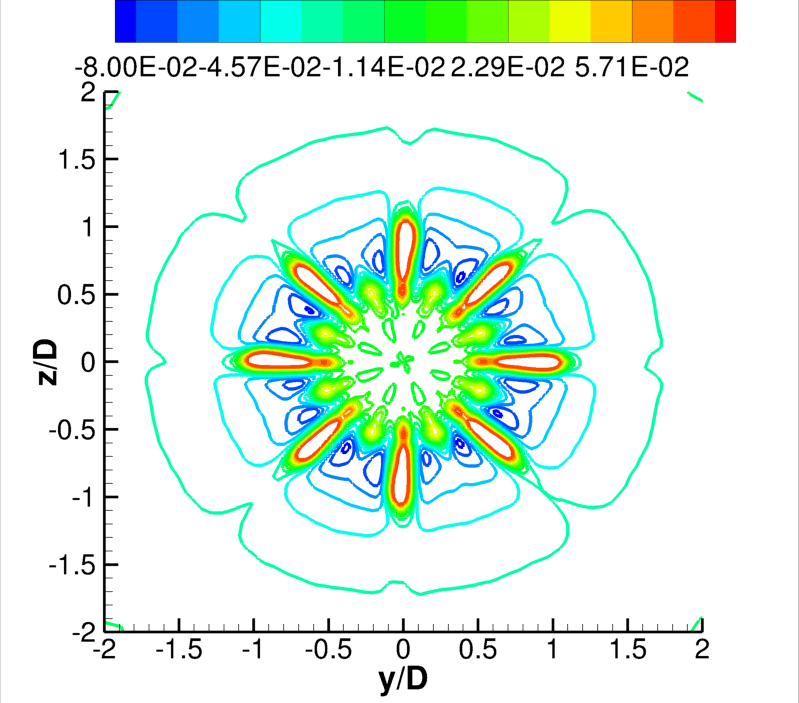
\includegraphics[width=3in]{M09ST025DT3x2vraxialcross}} %fixed
%%\subfloat[M=1.3, St=0.30, 20\% duty cycle]{\includegraphics[width=3in]{M13ST03x2vraxialcrossDuty20}} %fixe
%\end{centering}
%\caption{Cross-section of the phase-averaged ($\phi=0.1(2\pi)$) jet at an axial distance of 2D with contours of radial velocity}\label{CSvr}
%\end{figure}

%The effect of duty cycle on the hairpin structures in the controlled jets is more pronounced further downstream. Figure \ref{CSvrx4} depicts cross-stream slice of the phase-averaged radial velocity at an axial distance of 4D. At this axial location the low duty cycle subsonic case exhibits lower amplitudes of radial velocity signifying lower entrainment and thereby weaker hairpin vortices. The asymmetric structures (not shown) are also less coherent at this axial location for this duty cycle. This lower coherence is probably due to the thicker boundary layer at the exit which dampens the effects of the actuation and thereby creates a weaker structure that is unable to stay coherent throughout the entire potential core.
%\begin{figure} 
%\begin{centering}
%\subfloat[St=0.25, 10\% duty cycle]{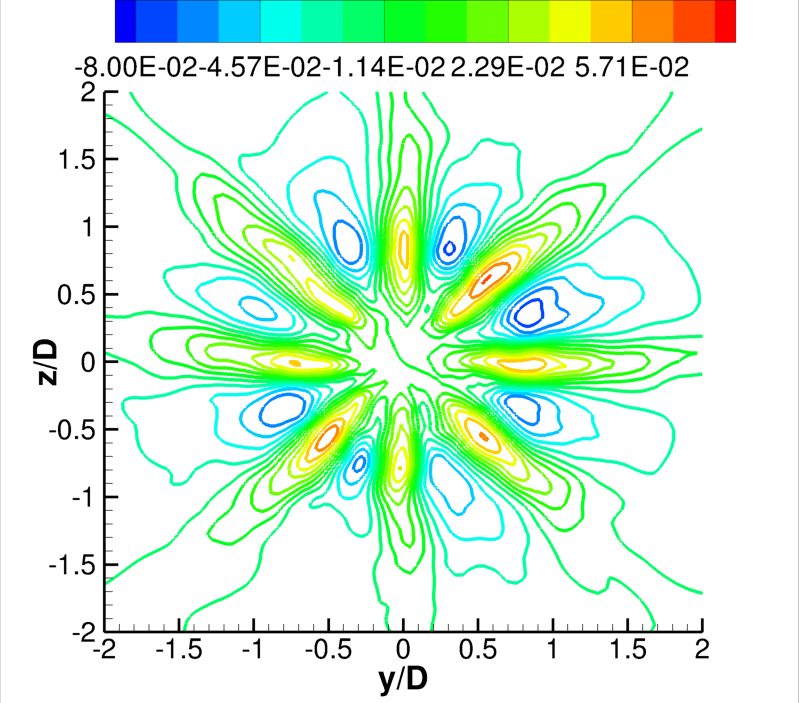
\includegraphics[width=3in]{M09ST025x4vraxialcros}} %fixed
%\subfloat[St=0.25, 3\% duty cycle]{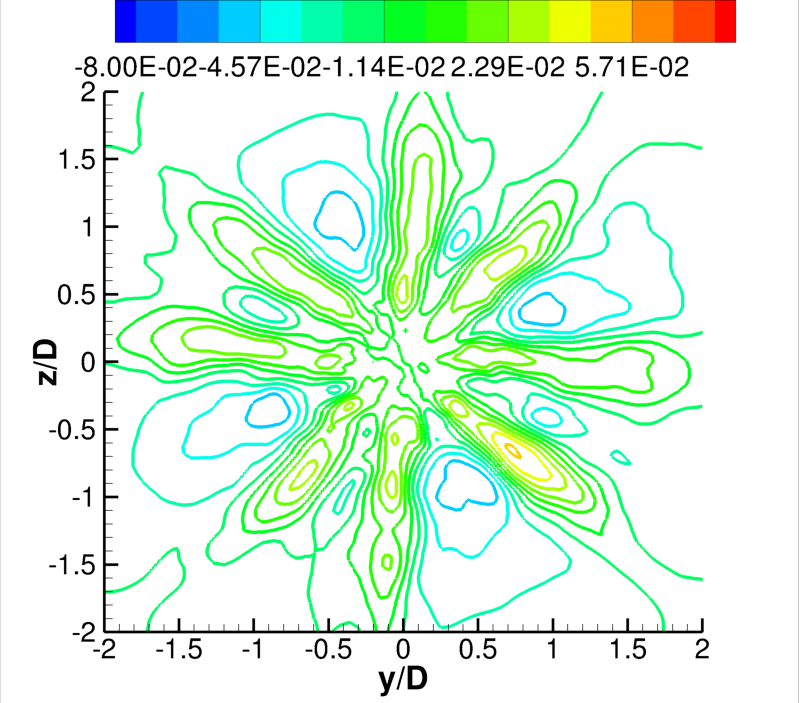
\includegraphics[width=3in]{M09ST025DT3x4vraxialcros}} %fixed
%%\subfloat[M=1.3, St=0.30, 20\% duty cycle]{\includegraphics[width=3in]{M13ST03x4vraxialcrossDuty20}} %fixe
%\end{centering}
%\caption{Cross-section of the phase-averaged ($\phi=0.1(2\pi)$) jet at an axial distance of 4D with contours of radial velocity}\label{CSvrx4}
%\end{figure}

The lipline phase-averaged pressure waveforms are now considered at $x/D=3$ in Fig. \ref{NUM_Phase_AVG_lip}a for each excitation frequency. The impulse response ($St=0.05$) has a peak around the characteristic time of 5 and then a trough at $tU_{jet}/D=6$. Note that a small secondary peak is seen after the trough which is not as distinguished in the experiments. This maybe due to the actuation model or the laminar nature of the nozzle exit.
These peaks corresponds to the compressions and expansion from the coherent structures seen in Fig. \ref{fig:isolevels05} in which the structure is pushing fluid in front of it and behind it fluid is rushing in to fill the void the structure just left. This pressure field is similar to that of a uniform flow superimposed with a doublet. Note that the jitter outside this waveform is due to the low number of excitation periods averaged to obtain the phase-averaged waveform. If there were no computational constraints and this low frequency case was allowed to run for 100 excitation cycles the surrounding wiggles would disappear. The St=0.15 case is similar to  the St=0.05 case however the time between excitation pulses is significantly reduced. For the St=0.25 case, the structures are interacting with each other significantly. 

Figure \ref{NUM_Phase_AVG_lip}b depicts the impulse response and St=0.25 phase-averaged waveform and the linearly superimposed impulse response waveform at a frequency of St=0.25 at an axial location of 3D on the lipline. This superposition of the impulse response consists of adding the impulse response to itself at a phase difference equal to that of the period of the St=0.25 case. 
The linear superposition on the lipline predicts the waveform shape and amplitude reasonably well. 
While the linear superposition does produce a secondary compression peak, it is far less prominent. Given the much greater amplitude of the pressure fluctuations along the jet lipline as compared to the irrotational near-field, it is perhaps unsurprising that nonlinear effects play a greater role. However, the interaction between the structures still appears to be governed predominantly by quasi-linear dynamics. This confirms the nearfield linear superposition findings of Refs. \cite{sinha2013} and \cite{Crawley2014} and extends it to the actual coherent structures.     
\begin{figure}
	\centering{}\subfloat[Phase averaged waveforms]{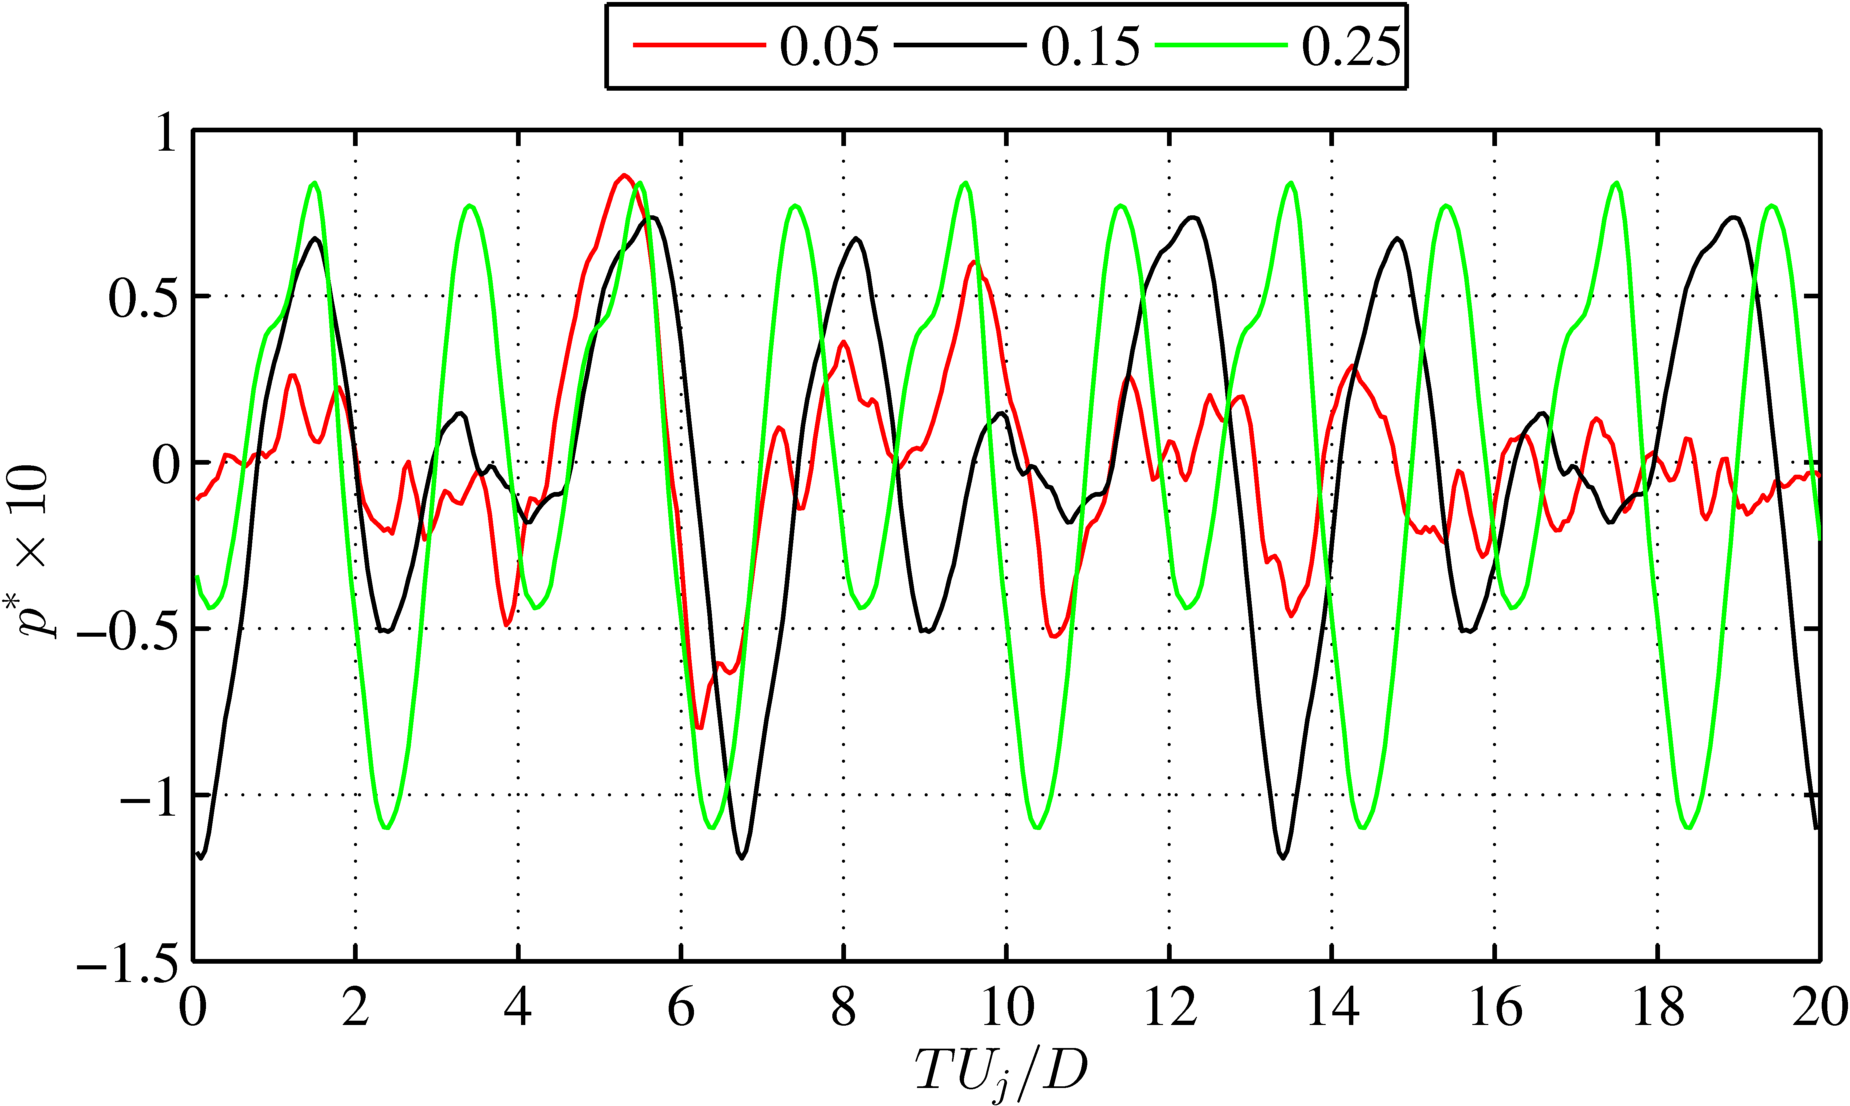
\includegraphics[width=3.25in]{Num_Phavg_x3D_lipline_corrected.png}
	}\subfloat[Linear superposition of the impulse response with St=0.25 waveform]{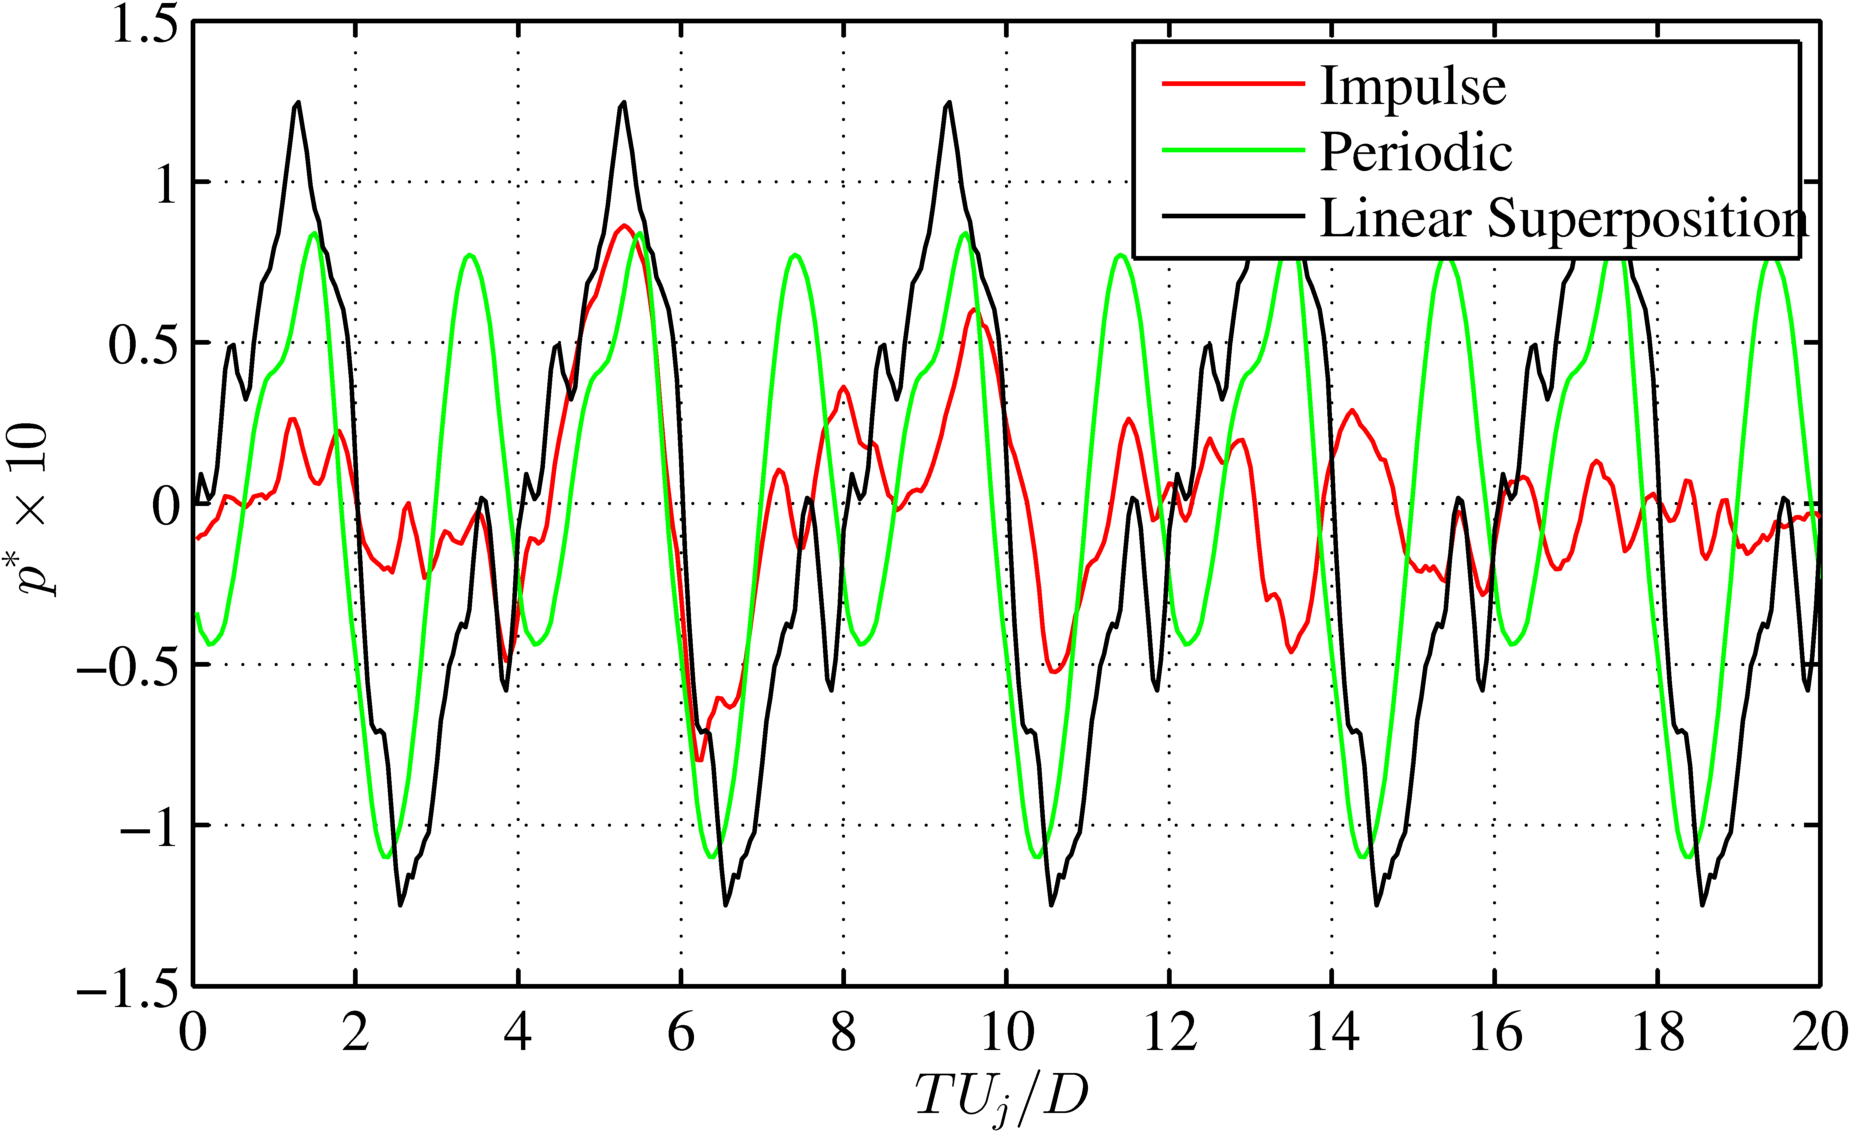
\includegraphics[width=3.25in]{Num_LnrPos_x3D_lipline_corrected.png}
}\caption{Lipline waveforms and superposed waveforms at $x/D = 3$, $r/D = 0.5$ for Mach 0.9}\label{NUM_Phase_AVG_lip}
\end{figure}

Looking at the autocorrelations of the nearfield points along the lipline can confirm the visual findings of the coherence of the structures in Figs. \ref{fig:isolevels05}-\ref{fig:isolevels}. 
Therefore, Fig. \ref{coherenceMach} depicts the autocorrelations of pressure at x/D=2 and 4 on the lipline. 
At $x/D=2$, the subsequent correlation peaks located at every excitation period increase in amplitude with increasing excitation frequency. This higher correlation value indicates a higher coherence in time at this spatial location. 
Further downstream (x/D=4), the subsequent correlation peaks are lower at all excitation frequencies than the upstream location indicating lower temporal coherence at this axial position. 
The bumpy appearance of the coherent structures (Figs. \ref{fig:isolevels05,fig:isolevels15,fig:isolevels}) implies that the structure is significantly changing each excitation period at this axial location. 

%%%INTEGRAL TIME SCALES FROM AUTOCORRELATIONS?????????
\begin{figure} 
\begin{centering}
\subfloat[St=0.05]{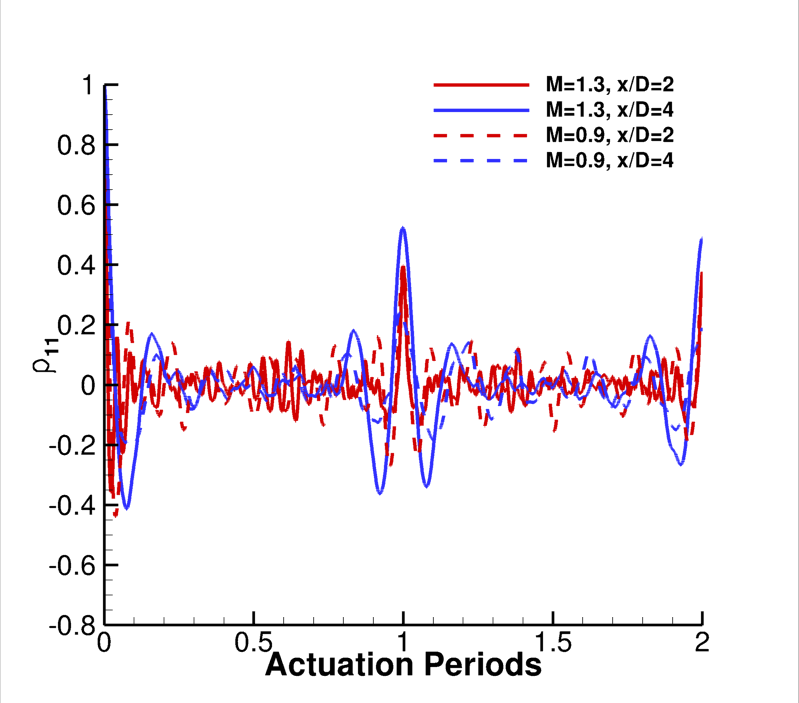
\includegraphics[width=3in]{MachsST005x2and4liplineauto}} %fixed
\subfloat[St=0.15]{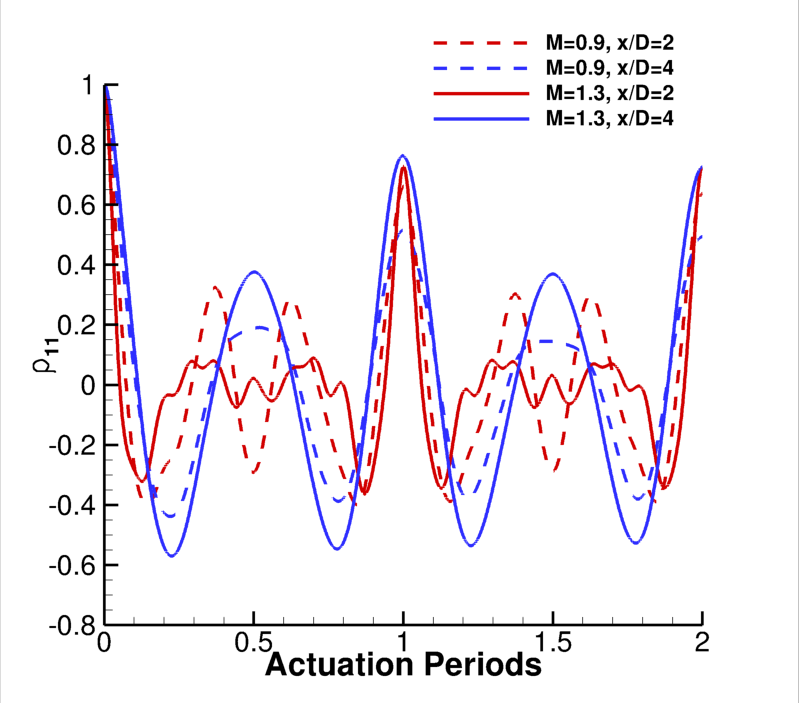
\includegraphics[width=3in]{MachsST015x2and4liplineauto}} %fixed

\subfloat[St=0.25]{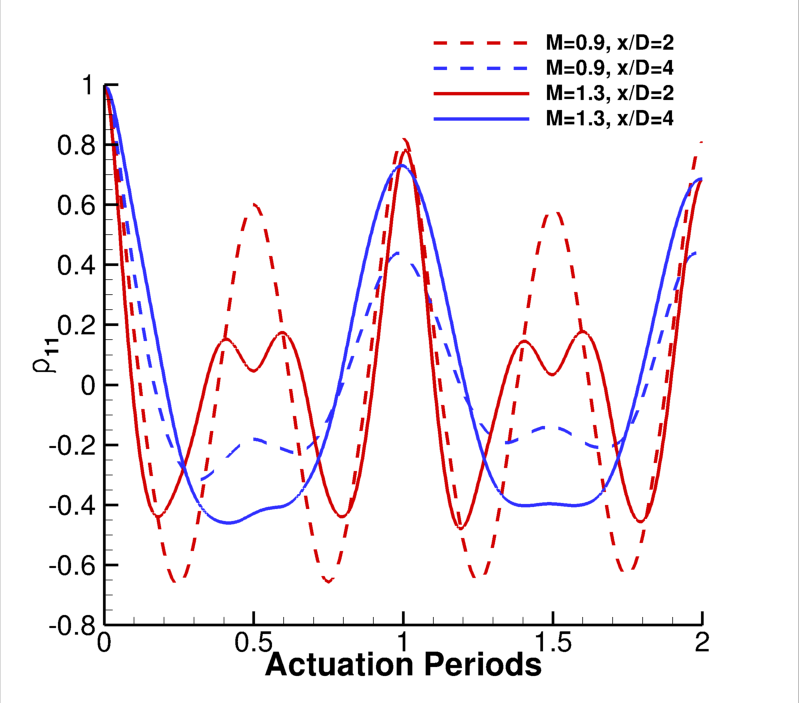
\includegraphics[width=3in]{MachsST025x2and4liplineauto}} %fixed
\end{centering}
\caption{Auto-correlation of the lipline pressure}\label{coherenceMach}
\end{figure}
%AZIMUTHAL DECOMP??????

Figure \ref{liplineconvec} depicts the correlations between different points along the lipline to illustrate the convective velocity of the structures and the spatial coherence of the structures. 
The convective velocities of each case and axial position were computed from Fig. \ref{liplineconvec} and displayed in Table \ref{tab:nearnozzleconvec} for near the nozzle exit and for near the end of the potential core. 
 %%%%%%%%%%%MAYBE NOT!!!!??? Check correlations shouldnt the a subsonic be slower at the end of the potential core due to all that extra entrainment?
\begin{figure} 
\begin{centering}
\subfloat[St=0.05]{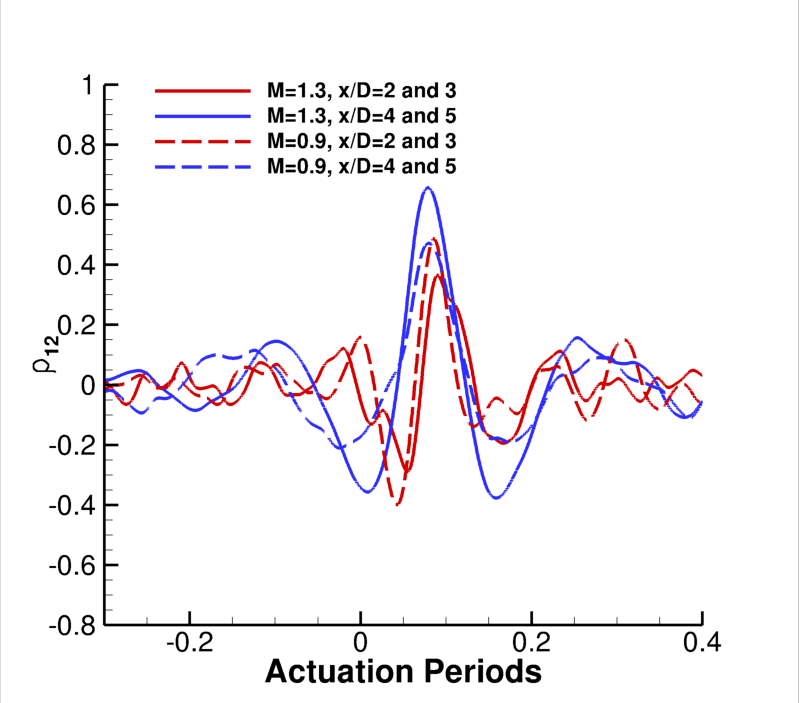
\includegraphics[width=3in]{corrliplineMAchSt005}} %fixed
\subfloat[St=0.15]{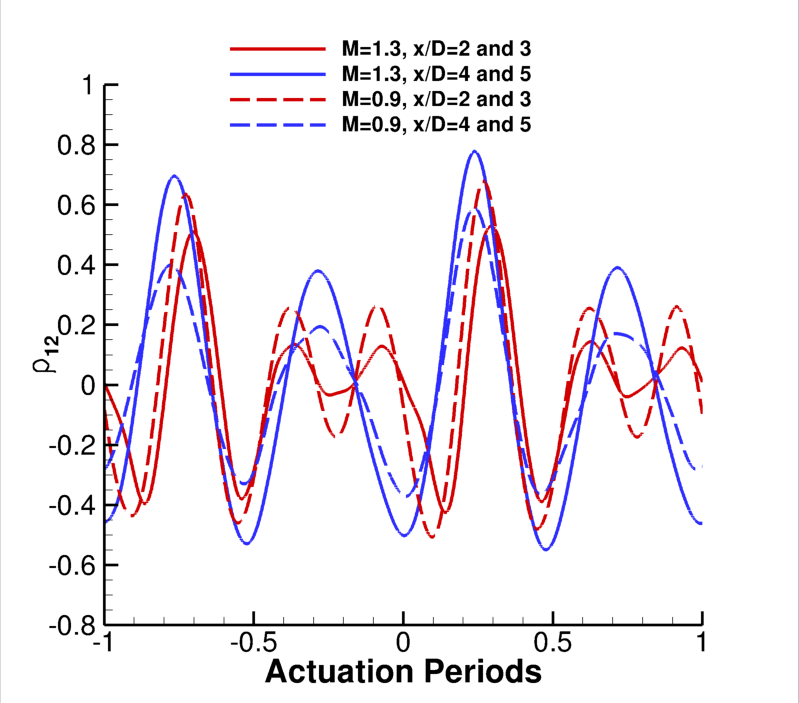
\includegraphics[width=3in]{corrliplineMAchSt015}} %fixed

\subfloat[St=0.25]{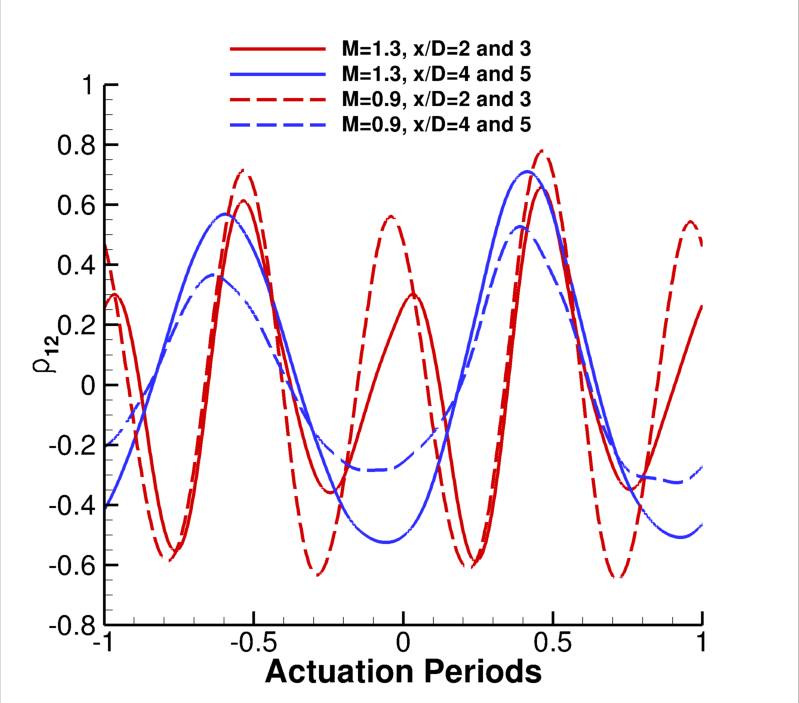
\includegraphics[width=3in]{corrliplineMAchSt025}} %fixed
\end{centering}
\caption{Two point correlations of the lipline pressure}\label{liplineconvec}
\end{figure}

\begin{center}
	\begin{tabular}{|l|l|l|l|l|l}
		 & No excitation & St=0.05 & St=0.15 & St=0.25 \\
		x/D=1 and 2 & 177 ($0.62U_{jet}$) & 165 ($0.58U_{jet}$) & 159 ($0.55U_{jet}$) & 152 ($0.54U_{jet}$) \\
		x/D=2 and 4 & 195 ($0.68U_{jet}$) & 181 ($0.63U_{jet}$) & 179 ($0.63U_{jet}$) & 182 ($0.64U_{jet}$) \\
	\end{tabular}
	\captionof{table}{Convective velocities from two-point correlations on the lipline}
	\label{tab:nearnozzleconvec}
\end{center}
The jet is consistently increasing in convective velocity with axial distance for each case.
Therefore, the jet is entraining more core flow fluid near the nozzle exit which increases the convective velocity. Further downstream, the ratios indicate that the entrainment is more evenly distributed between the high speed side and the low speed side.

%%%%%%%%%%%%%%%%%%%%%%%%%%%%%%%%%%%%%%%%%%%%%%%%%%%%%%%%%%%%%%%%%%%%%%%%%%%%%%%%%%%%%%%%%
\subsection{Connecting the Large Scale Structures to the Hydrodynamic Near-field}
The coherent structures presented previously in Section \ref{structure} cause disturbances in the near-field that can be seen in the near field pressure data.
\begin{figure}
\begin{center}
\begin{centering}
\subfloat[M=0.9, St=0.05]{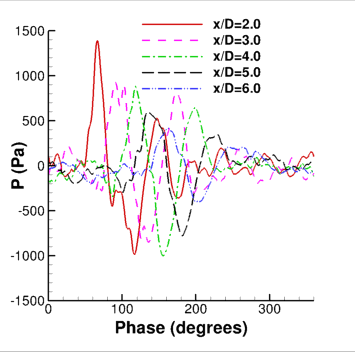
\includegraphics[width=2.5in]{M09phaseSt005fixed}}%fixed
\subfloat[M=0.9, St=0.15]{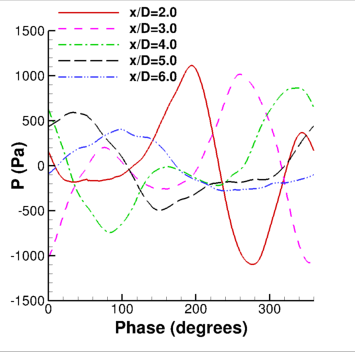
\includegraphics[width=2.5in]{M09phaseSt015fixed}}%fixed

\subfloat[M=0.9, St=0.25]{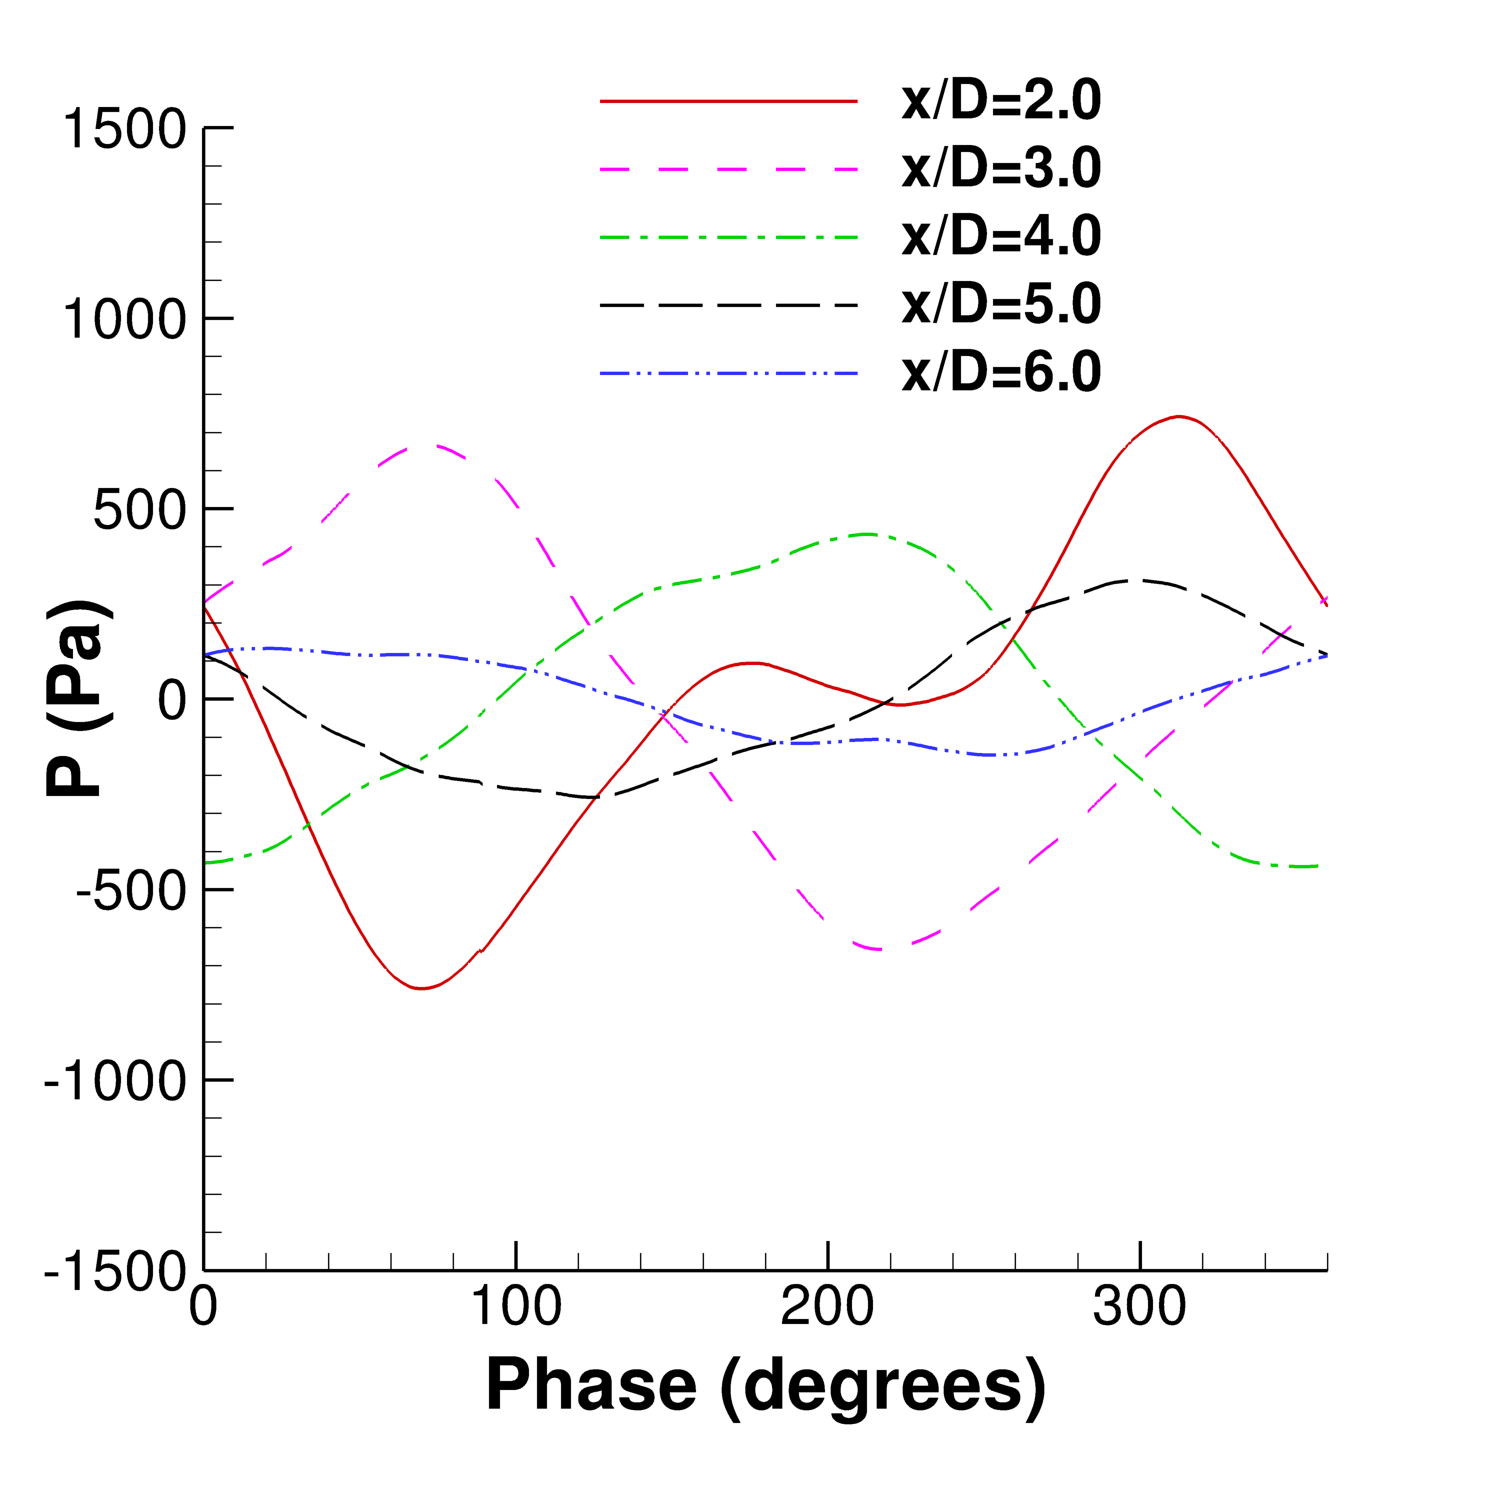
\includegraphics[width=2.5in]{M09phaseSt025}}%fixed
\end{centering}
\caption{Phase-averaged pressure waveforms of $Array~1$}
\label{fig:phaseaxialbothM}
\end{center}
\end{figure}
A more detailed analysis may be obtained through the study of the phase-averaged signal close to the shear layer.
Figure \ref{fig:phaseaxialbothM} depicts the phase-averaged point probe data along $Array~1$ for the different excitation frequencies. The x-axis is the phase in degrees within the cycle. The waves dampen out with increasing axial distance which is due to the short potential core that causes the structures to reach their maximum potential early in the jet (x/D=2). %entrainment and size of structures???
The propagation of the pulse is observed in the peaks which arise at
successive locations with increased phase. The low frequency case
($St=0.05$) depicts a long neutral period or "quiet" time between each
pulse. After the core length ($x/D=5$), the pulses are wider and no
longer exhibit a sharp peak.
As the excitation frequency increases and the actuator induced waves interact with each other more the amplitude of the waveforms decrease. This can be attributed to the linear superpositioning discussed for the lipline earlier (Section \ref{compresscontrol}) and will be discussed further in regard to the nearfield later in this chapter. 
For each frequency, the phase-averaged waves are hydrodynamically dominated due to the proximity of the probes to the shear layer. However, embedded in this signal is the acoustic response which will propagate to the farfield. This acoustic response can be separated from the hydrodynamic response through a wavelet method described and implemented in Ref. \cite{Crawley2015} for a subsonic jet were there is a significant difference between the speed of the acoustic waves.  

These nearfield phase-averaged waveforms can be connected to the coherent structures depicted in Figs. \ref{fig:isolevels05} to \ref{fig:isolevels} and the pressure responses of the structures in Fig. \ref{NUM_Phase_AVG_lip}a.
The phase averaged structures of $St=0.05$ in
Fig.~\ref{fig:isolevels05} depict a quiet time at an axial distance of $x/D=2$
and $4$ for the phase of $0.1(2\pi)$. This corresponds, at these
locations, to the neutral period observed in Figs.~\ref{fig:phaseaxialbothM}a and b for
a phase angle of $36^o$.  With increase in phase, the structure moves
to the right as observed in the succession of peaks in
Figs.~\ref{fig:phaseaxialbothM}a and b.  This corresponds to a convective
velocity of $0.63U_{jet}$ between $x/D\sim 1$ and $x/D\sim 2$. This differs from the lipline convective velocities due to the increased influence of the acoustic waves outside the shear layer. This will be discussed more in terms of the two-point correlations.
The large hydrodynamic wave at $x/D\sim 1$ at
$0.1(2\pi)$ phase in Fig.~\ref{fig:isolevels05} has just passed the axial
distance of $x/D=5$ (viewing range of the iso-level structures) at the
$\phi=0.6(2\pi)$ phase leaving the axial point in the top of the secondary compression peak. This corresponds to the smaller secondary peak at
$x/D=5$ at $216^o$ in Figs.~\ref{fig:phaseaxialbothM}a and b.

For $St=0.15$, the phase averaged signal at axial positions shown in
Figs.~\ref{fig:phaseaxialbothM}c and d, indicates that the ``quiet'' time between
pulses becomes shorter with downstream distance of the probe.  This
also corresponds with the increasing size of the structures in the jet. At an
axial distance of $x/D=4$, the horizontal neutral part of the phases
is minimal, suggesting that the subsequent structure interaction is occuring. This location also has the
highest amplitude phase averaged wave for the supersonic case.  Correlating to
Fig.~\ref{fig:isolevels15} for the $St=0.15$ case, the $x/D=4$ location at 
$0.1(2\pi)=36^\circ$ phase shows a large dilation wave associated with
a well-developed roller. Clearly, the growth of the rings with
distance from the nozzle exit corresponds to increasingly shorter
quiet times at downstream probes: an effect clearly observed in
Fig.~\ref{fig:phaseaxialbothM}c and d.  Thus, at $0.1(2\pi)$ phase, $x/D=2$ has
significant quiet time while at $x/D=6$ the pulses essentially merge
with each other to create a sine-like response.

For the $St=0.25$ supersonic case, the first axial position plotted has a sine-like wave indicating significant structure interactions. The subsonic case does not exhibit this sine-like state yet at this axial location due to the more prominent secondary compression wave that is seen in the impulse response at this location. The waves maintain a sine-like pattern beyond $x/D=2$ even after the potential core ($x/D=5.5$). 

Figure \ref{fig:isolevels} can be used to give a visual understanding of these phase-averaged pressure probes for the St=0.25 cases. In Fig. \ref{fig:isolevels}, the white dilatation waves correspond to an increase in pressure while the black dilatation waves correspond to a decrease in pressure. At a phase of $\phi=0.1(2\pi)=36^\circ$ in Fig. \ref{fig:isolevels}a, the $x/D=4$ point probe is entering a white dilatation region (increase of pressure) while the x/D=2 probe is entering a black dilatation wave corresponding to a decrease in pressure. In Fig. \ref{fig:phaseaxialbothM}a, an increase of pressure is seen at $x/D=4$ and a decrease is seen at $x/D=2$ for the phase of $36^\circ$. At a phase of $\phi=0.6(2\pi)=216^\circ$, the $x/D=2$ location is in the region of pulse interactions where structure B and A' are beginning to merge. This area translates to a bumpy uphill region for $x/D=2$ in Fig. \ref{fig:phaseaxialbothM}c. After the two structures (A' and B) merge ($\phi=0.1(2\pi)$) around an axial distance of $3D$, the phase averaged point probe depicts a wiggle in the increasing pressure. 

%\begin{figure*} 
%\begin{centering}
%\subfloat[x/D=2]{\includegraphics[width=3.5in]{}}
%\subfloat[x/D=5]{\includegraphics[width=3.5in]{}}
%\subfloat[x/D=10]{\includegraphics[width=3.5in]{}}
%\end{centering}
%\caption{Auto-correlation of the near field pressure for the first array}\label{Autocorrel}
%\end{figure*}
\begin{figure} 
\begin{centering}
\subfloat[St=0.05]{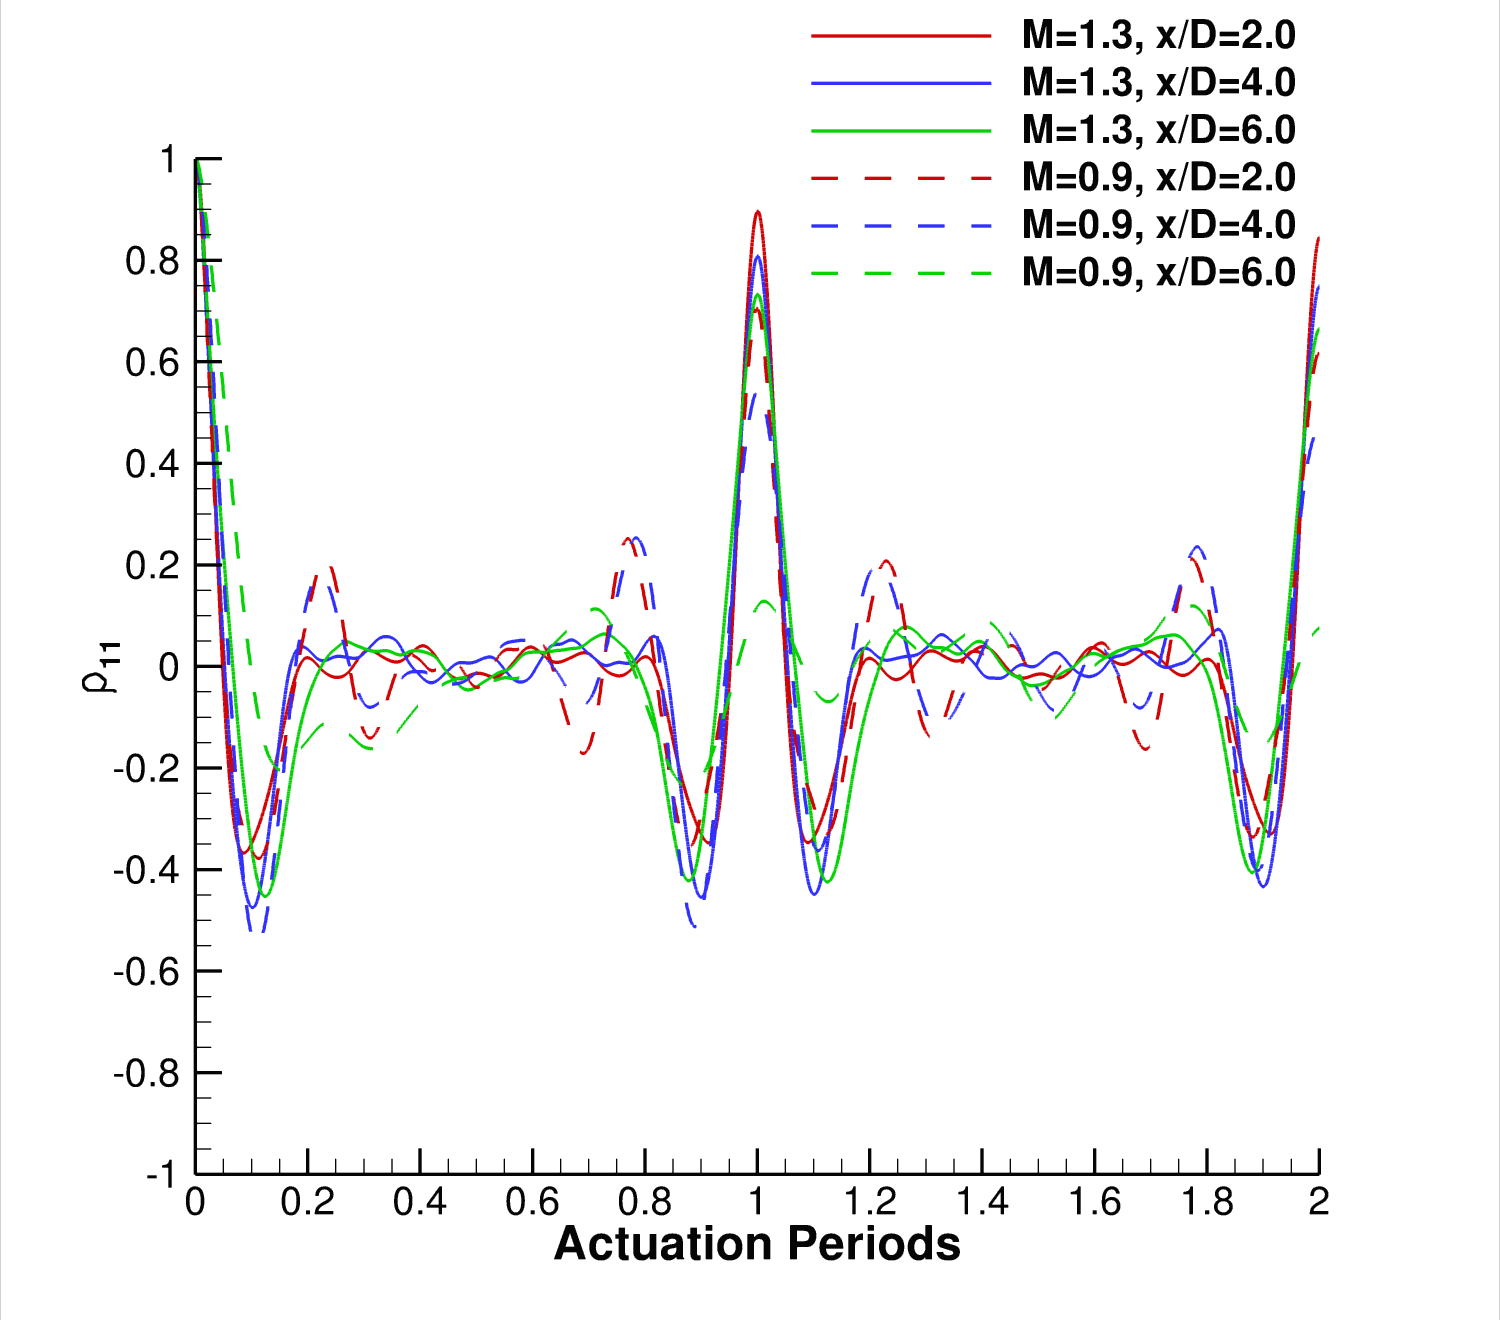
\includegraphics[width=3in]{M09M13autocorrarray1ST005}} %fixed
\subfloat[St=0.15]{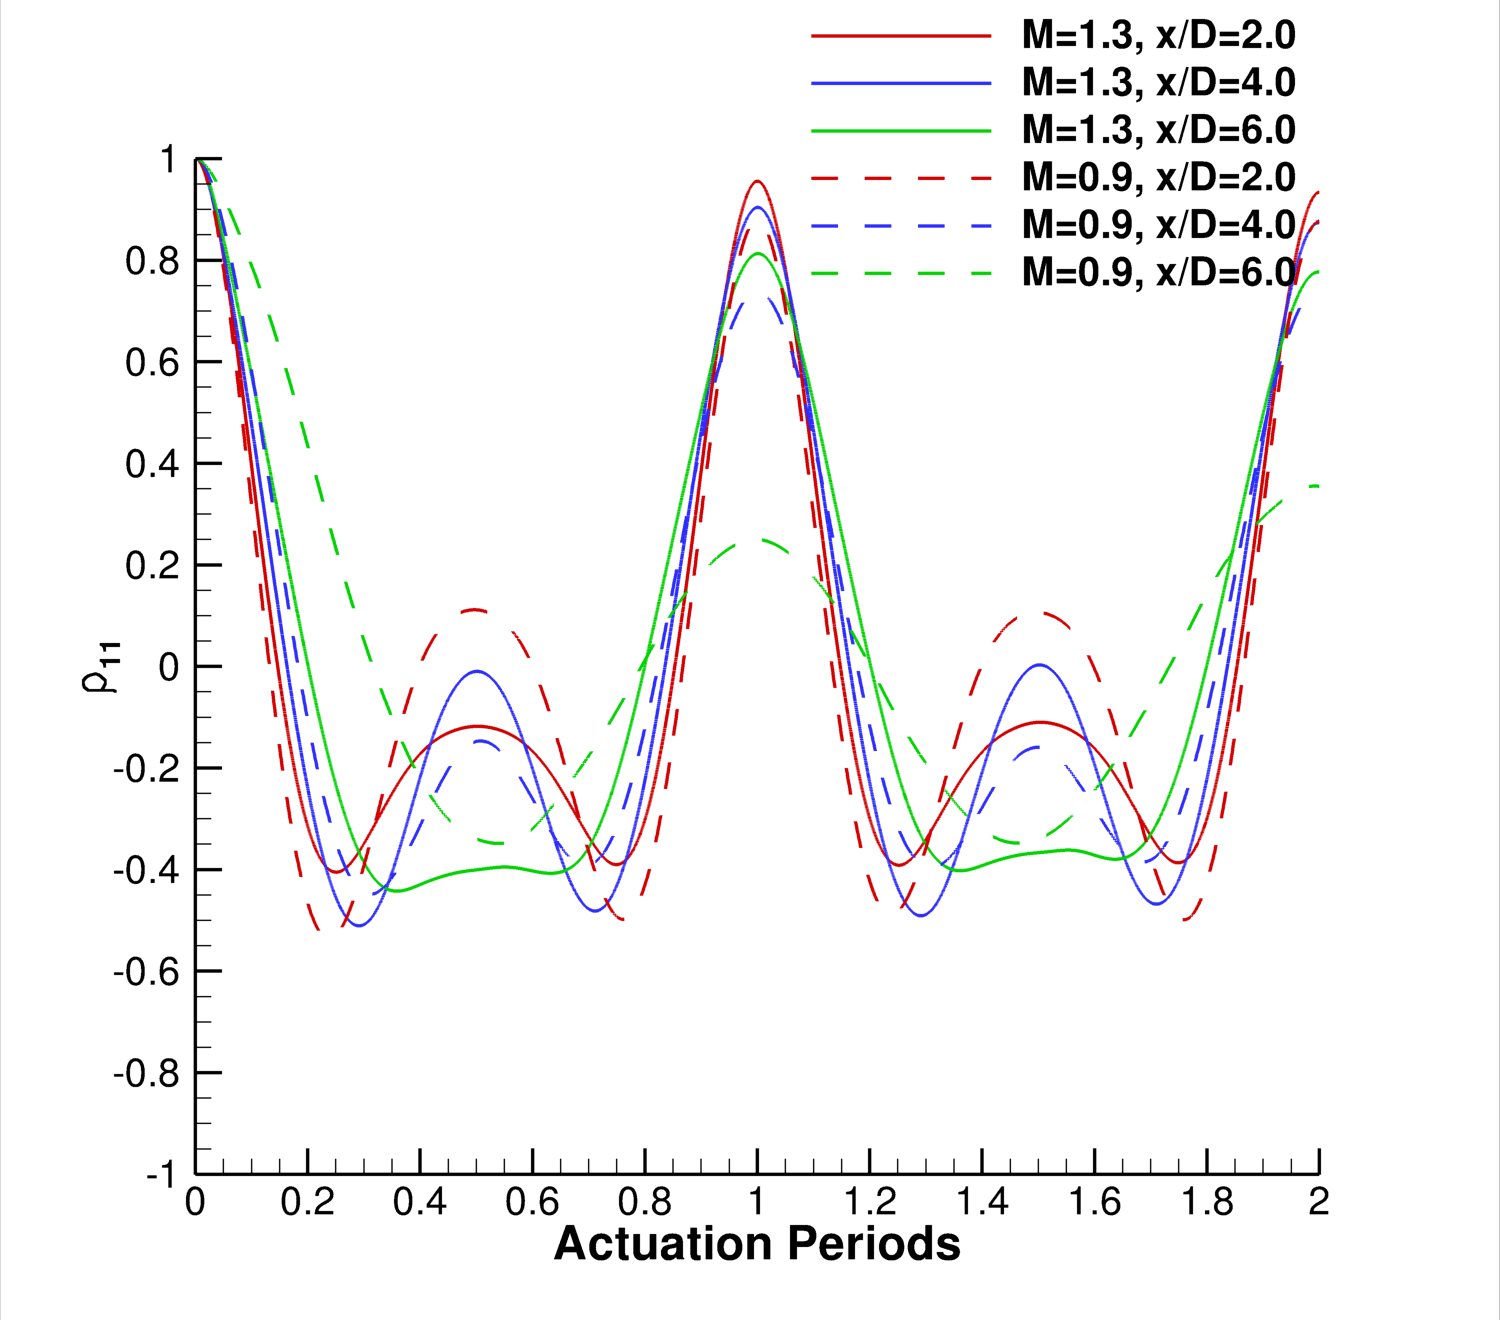
\includegraphics[width=3in]{M09M13autocorrarray1ST015}} %fixed

\subfloat[St=0.25]{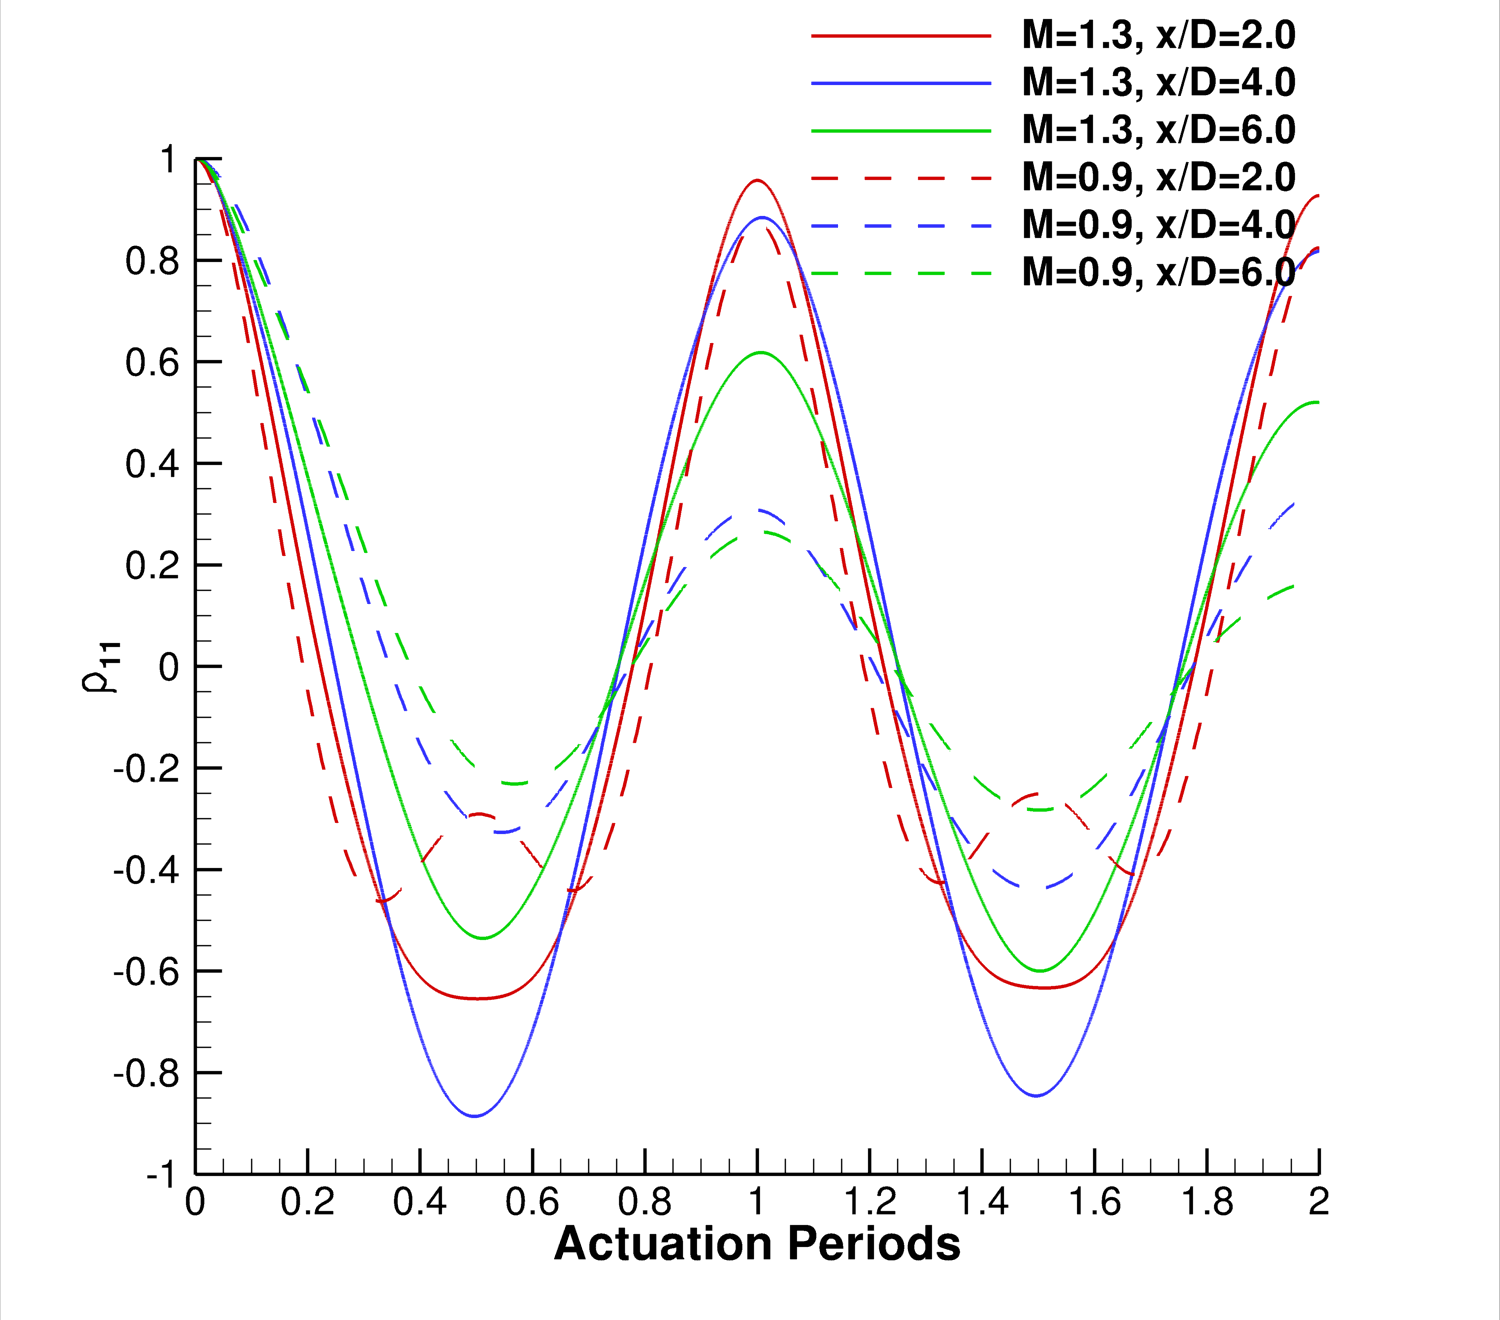
\includegraphics[width=3in]{M09M13autocorrarray1ST025}} %fixed
\end{centering}
\caption{Auto-correlation of the near field pressure for the first array}\label{Autocorrel}
\end{figure}
%\begin{figure*} 
%\begin{centering}
%\subfloat[St=0.05, Mach 0.9]{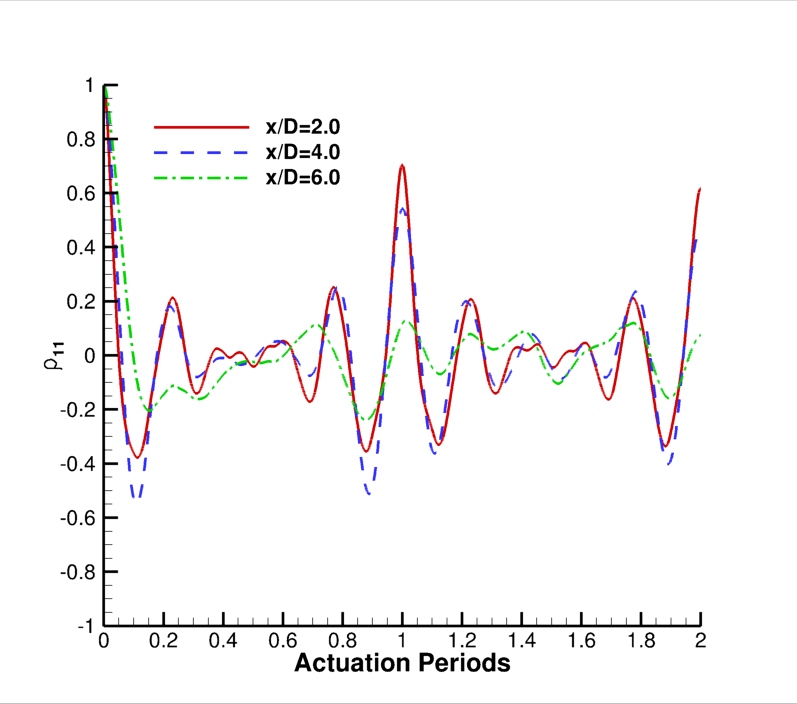
\includegraphics[width=3in]{M09autocorrarray1ST005}} %fixed
%\subfloat[St=0.05, Mach 1.3]{\includegraphics[width=3in]{autoarray1ST005.png}}
%\subfloat[St=0.15, Mach 0.9]{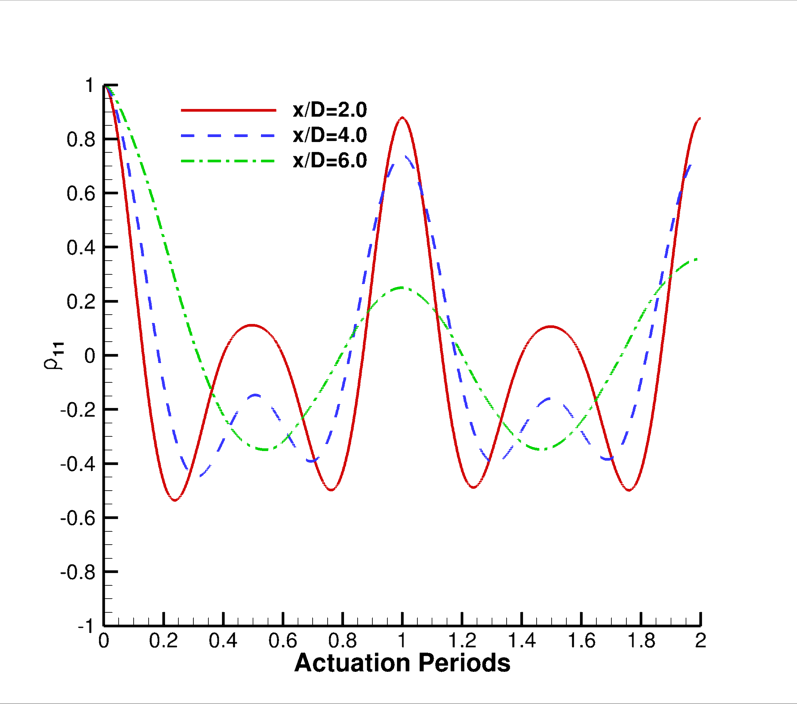
\includegraphics[width=3in]{M09autocorrarray1ST015}} %fixed
%\subfloat[St=0.10, Mach 1.3]{\includegraphics[width=3in]{autoarray1ST015.png}}
%\subfloat[St=0.25, Mach 0.9]{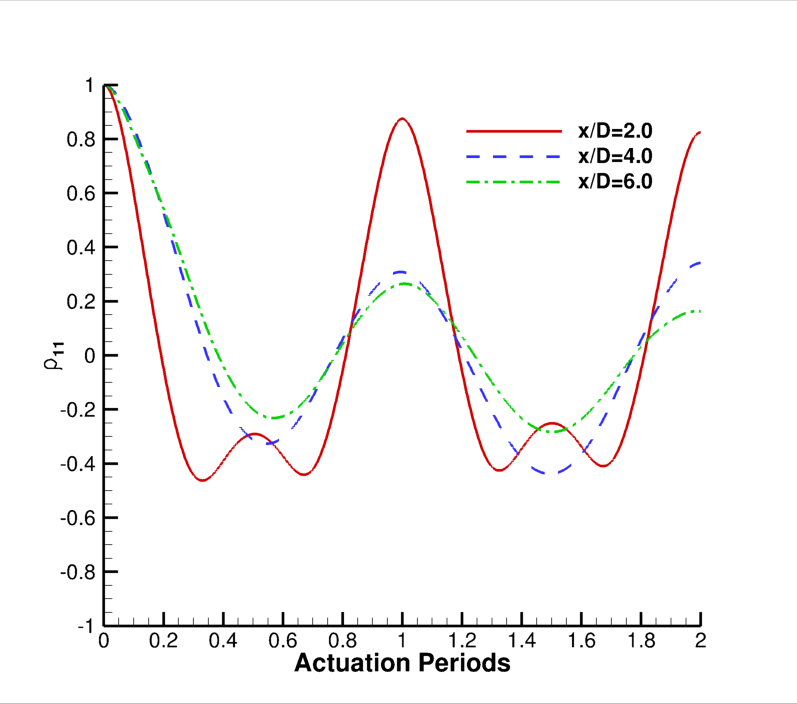
\includegraphics[width=3in]{M09autocorrarray1ST025}} %fixed
%\subfloat[St=0.25, Mach 1.3]{\includegraphics[width=3in]{autoarray1ST025.png}}
%\end{centering}
%\caption{Auto-correlation of the near field pressure for the first array}\label{Autocorrel}
%\end{figure*}
Figure \ref{Autocorrel} depicts the auto-correlations of pressure for the first array for each excitation case at both Mach numbers. The peak correlations decrease with axial distance as more fluid is entrained modifying subsequent structures in different ways and the jet becomes more turbulent. The axial positions beyond the potential core show the greatest reduction in correlation. This enhanced decay in correlation is also seen in the experimental results at Mach $0.9$ (Alkandry \etal \cite{Alkandry2013}). This indicates that the hydrodynamically dominated nearfield of the subsonic jet has very little temporal coherence which implies that the waves passing through these points are changing significantly from excitation period to excitation period. This change could be due to a combination of effects including: the entrainment seen by the jet which would altar each structure differently and the higher turbulence with axial distance.

Figure \ref{Autocorrel}a depicts the low excitation frequency autocorrelations. For the points within the potential core, the correlation value quickly drops below zero with increasing lag until a phase of $0.1(2\pi)$. Beyond this phase, the axial positions of $2D$ and $4D$ maintain significant correlation values except for the range in between each period of $0.4(2\pi)$ and $0.6(2\pi)$. In general for all excitation frequencies, the integral time scale increases with axial distance as the structures in the shear layer become larger  or resultant waves from the coherent structures on the lipline decrease their convective velocity. Beyond the potential core, the hydrodynamically dominated waves are moving at a slower speed than in the potential core region. The convective velocities will be discussed further in regards to the two-point correlations. 

The $St=0.15$ case (Fig. \ref{Autocorrel}b) depicts a secondary smaller hump located in between each excitation period for the points within the potential core. This rise between periods is similar to removing most of the zero correlation region between the actuation periods in the impulse response autocorrelations and signifies the beginnings of subsequent structure interactrions. Beyond the potential core at an $x/D=6.0$ a trough is present. %Referring back to Fig. \ref{fig:phaseaxialbothM}b, 

The high frequency cases in Fig. \ref{Autocorrel}c, exhibit a sine-pattern inside the potential core region ($x\leq5.5D$) with peaks at intervals corresponding to the excitation frequency except for the $x/D=2$ location. This location has a hump at the half period indicating the beginning of structure interaction. After the potential core, the correlation values decay slowly to zero throughout time. A decrease in subsequent period peaks is seen with axial distance. This decrease in peak correlation values with axial distance is due to the decrease in organization of large scale structures beyond the potential core and thereby organization of the surrounding nearfield. %explain the isolevels for this stuff

%?????????????REDO PLOTS SO THE upstream peaks are on the left side of zero and the downstream peaks on the right side of zero!!!!!!!!!!!!
\begin{figure} 
\begin{centering}
\subfloat[No control]{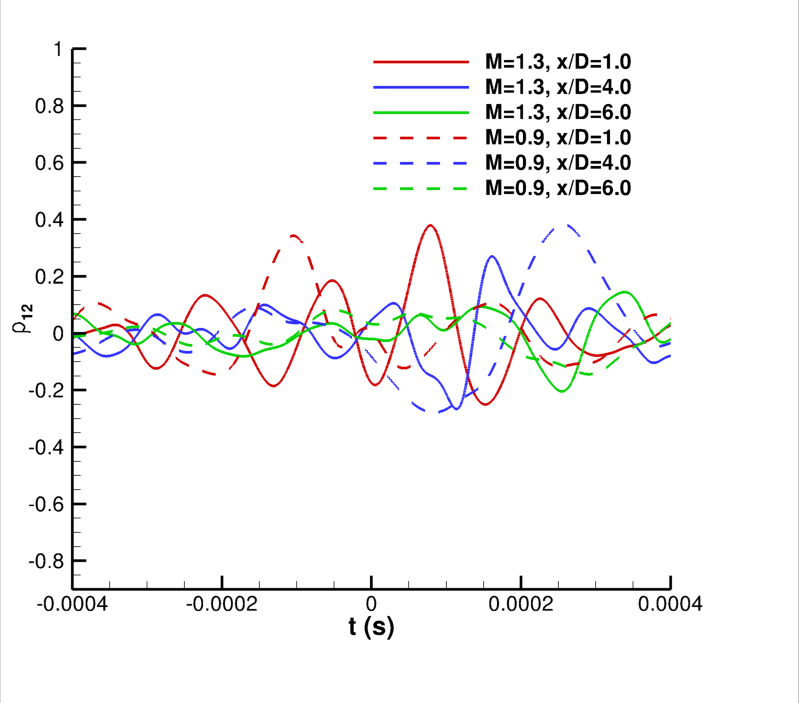
\includegraphics[width=3in]{M09M13crosscorrNE}}%WHAT IS WRONG WITH THE SUPERSONIC CASE??
\subfloat[St=0.05]{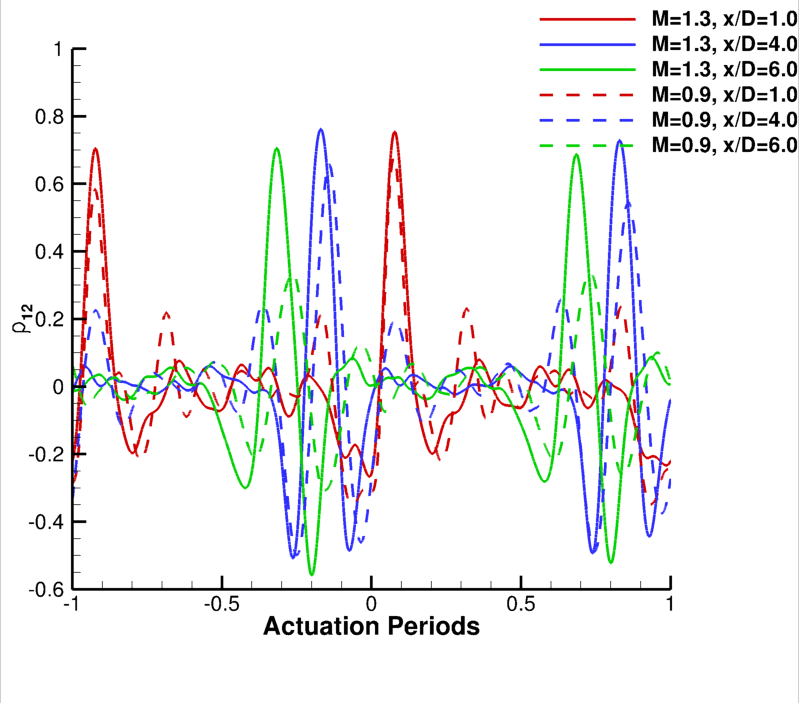
\includegraphics[width=3in]{M09M13crosscorrSt005}}

\subfloat[St=0.15]{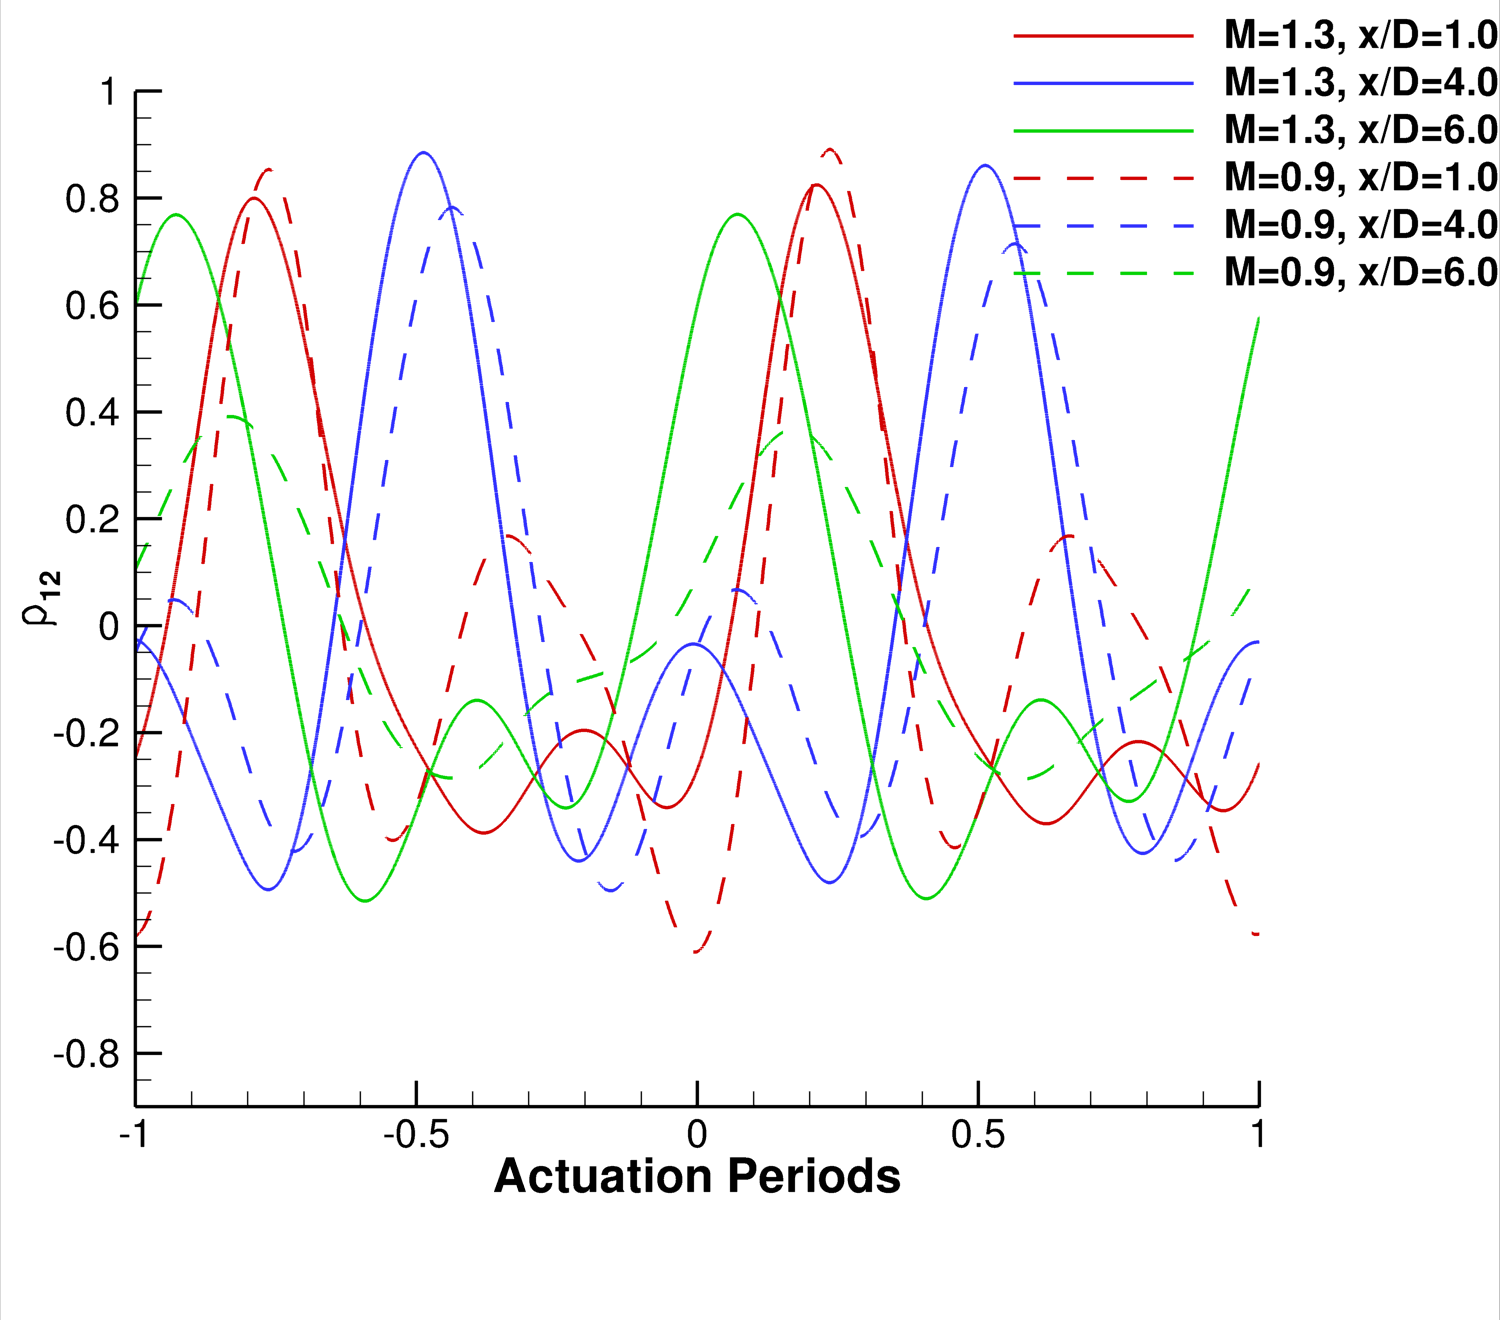
\includegraphics[width=3in]{M09M13crosscorrSt015}}
\subfloat[St=0.25]{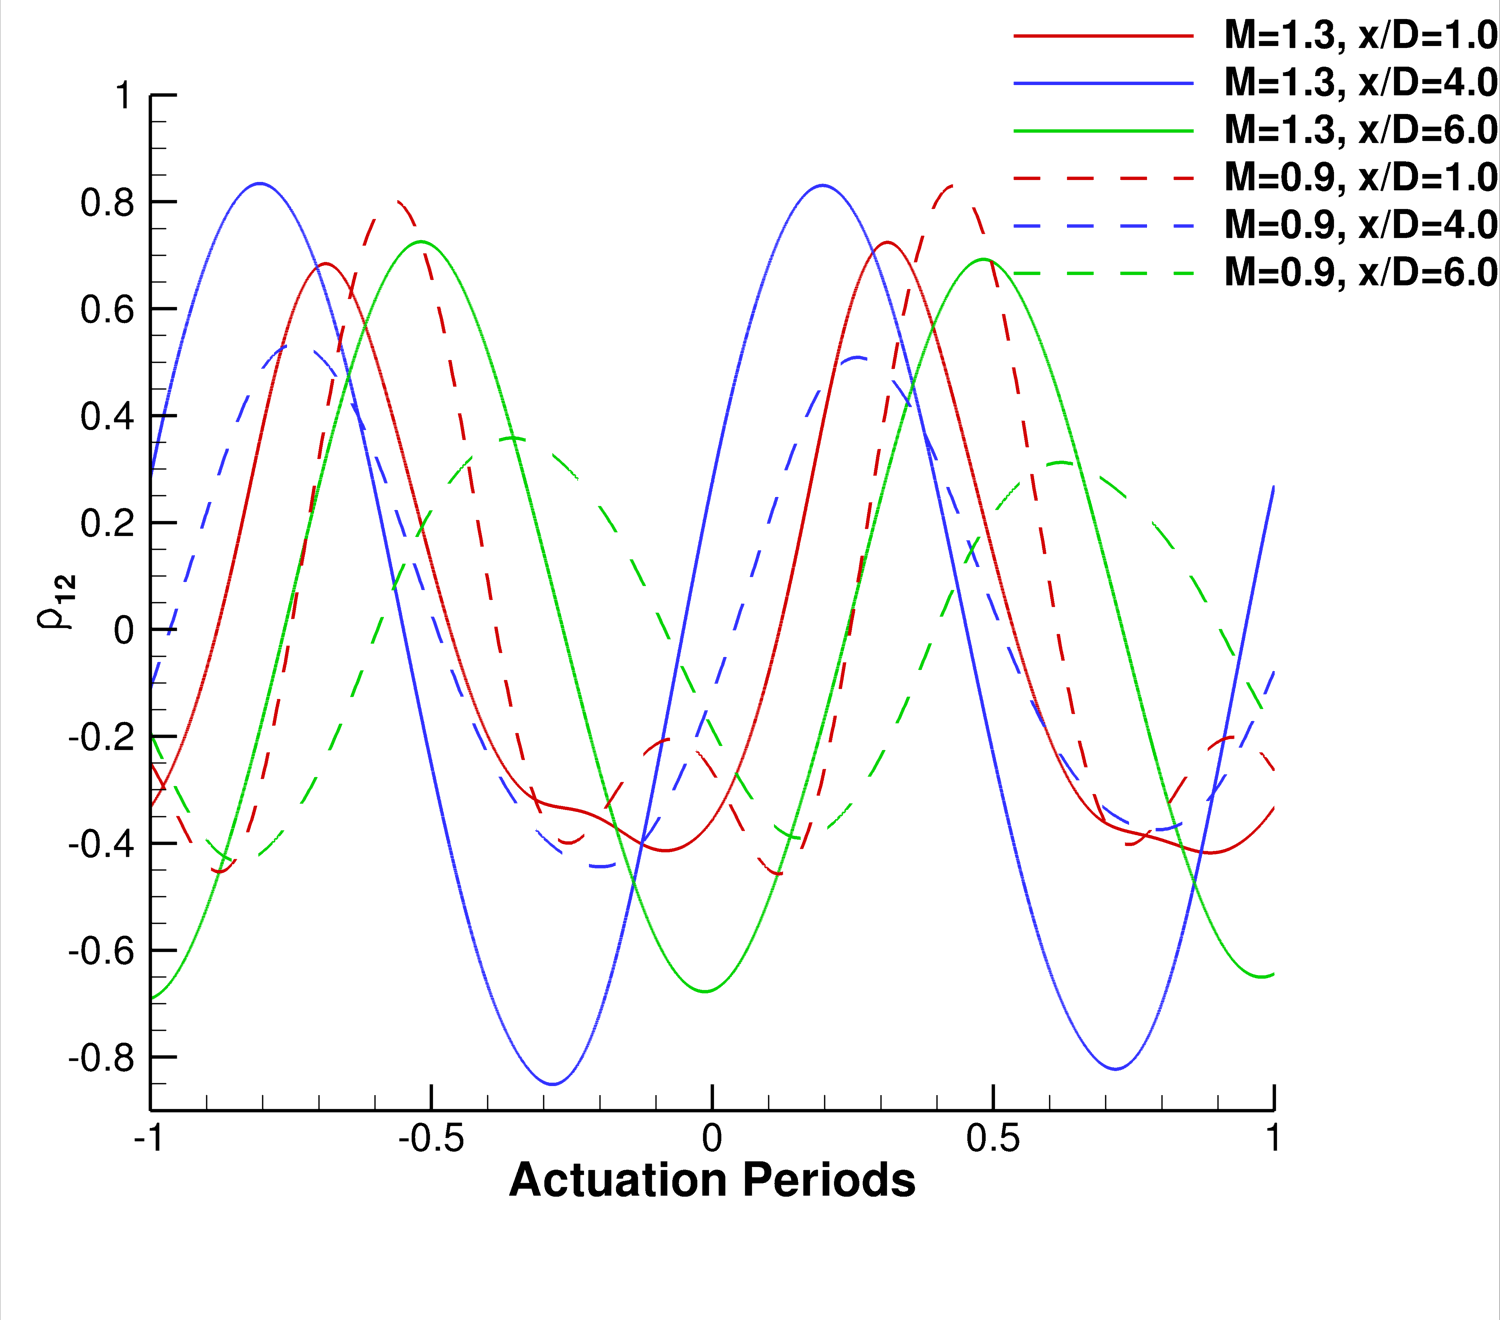
\includegraphics[width=3in]{M09M13crosscorrSt025}}
\end{centering}
\caption{Two-point correlation of the near field pressure for the first array with x/D=2 and r/D=1.355}\label{2ptCorrel}
\end{figure}
%\begin{figure*} 
%\begin{centering}
%\subfloat[St=0.05, Mach 0.9]{\includegraphics[width=3in]{M09crosscorrarray1ST005}}
%\subfloat[St=0.05, Mach 1.3]{\includegraphics[width=3in]{cross2xdST0051to1.png}}
%\subfloat[St=0.15, Mach 0.9]{\includegraphics[width=3in]{M09crosscorrarray1ST015}}
%\subfloat[St=0.15, Mach 1.3]{\includegraphics[width=3in]{cross2xdST0151to1.png}}
%\subfloat[St=0.25, Mach 0.9]{\includegraphics[width=3in]{M09crosscorrarray1ST025}}
%\subfloat[St=0.25, Mach 1.3]{\includegraphics[width=3in]{cross2xdST0251to1.png}}
%\end{centering}
%\caption{Two-point correlation of the near field pressure for the first array with x/D=2 and r/D=1.355}\label{2ptCorrel}
%\end{figure*}
Figure \ref{2ptCorrel} portrays the two-point correlations of pressure comparing the first array point probes to the $x/D=2$ location on the first array. For the impulse response case (Fig. \ref{2ptCorrel}a), the correlations decay rapidly with axial distance. 
This shows that not only that there is low temporal coherence (see Fig. \ref{Autocorrel}) but also that there is low spatial coherence; meaning the structure changes significantly as it propagates downstream. 
The $St=0.15$ case (Fig. \ref{2ptCorrel}b) exhibits a more sine like pattern with the characteristic hump seen in the autocorrelations which likewise indicates structures beginning to interact in the shear layer.
 For a phase difference of $0.5(2\pi)$ in the $St=0.15$ cases, a high correlation value is seen for the 4D axial location. Connecting this correlation to the coherent structures in Fig. \ref{fig:isolevels15} there is a dark dilatation wave (decrease in pressure) at the 4D location for the phase of $0.1(2\pi)$ and half a phase later, $0.6(2\pi)$, the 2D point is located in a dark dilatation region indicating a high correlation between these two points every half excitation period.  

The two-point correlations for the high frequency case (Fig. \ref{2ptCorrel}c) exhibit a sinusoidal response except for the first axial position shown ($x/D=1$). For an axial distance of $1D$, a high positive correlation is obtained half an excitation period away. 
Therefore, in Fig. \ref{fig:isolevels}a, when $x/D=2$ is encountering a white dilatation wave (increase in pressure) at a phase of $\phi=0.1(2\pi)$, $x/D=1$ will experience a white dilatation wave also half a period later ($\phi=0.6(2\pi)$). Similarly, a negative correlation value is observed for $x/D=1$ at a phase difference close to zero. Therefore, in Fig. \ref{fig:isolevels}a for a phase of $\phi=0.6(2\pi)$, the axial position of $1D$ has a black dilatation wave instead of the white dilatation wave that $x/D=2$ has for the same phase. As the structures break apart at the end of the potential core, these relationships also degrade. 
The peaks closest to zero in the two-point correlations have the highest maximums. Therefore, each structure will be more correlated to itself further downstream than to the previous/subsequent structures. This can be attributed to the random perturbations in the jet that adjust each actuated structure differently.
%more maybe?

\begin{center}
	\begin{tabular}{|l|l|l|l|l|l}
		 & No excitation & St=0.05 & St=0.15 & St=0.25 \\
		x/D=1 and 2 & 243 ($0.85U_{jet}$) & 188 ($0.66U_{jet}$) & 180 ($0.63U_{jet}$) & 165 ($0.59U_{jet}$) \\
		x/D=2 and 4 & 197 ($0.69U_{jet}$) & 202 ($0.71U_{jet}$) & 197 ($0.69U_{jet}$) & 192 ($0.67U_{jet}$) \\
	\end{tabular}
	\captionof{table}{Convective velocities from two-point correlations on Array 1}\label{tab:nearnozzleconvecarray}
\end{center}
The velocity of the waveforms surrounding the jet can be computed from the correlations of Fig. \ref{2ptCorrel} for the near field probes on Array 1 two investigate the change in convective velocity from the lipline (shown in Tables \ref{tab:nearnozzleconvec}) to the hydrodynamically dominated nearfield. Table \ref{tab:nearnozzleconvecarray} lists the average velocity of the waves between the axial point of 1D and 2D on Array 1 and the velocities of the waveforms that travel between x/D=2 and 4. These velocities are consistently higher than the convective velocities observed in Section \ref{structure} on the lipline but display similar trends. The hydrodynamic waves will decrease exponentially with radial distance away from the shear layer leaving the near field dominated by waves traveling at the speed of sound. Therefore, the velocities in the nearfield are higher than the convected structures in the shear layer due to the increasing influence of the acoustic waves. This is important to take into account for experimentalists who compute the convective velocity of the structures from the nearfield due to limitations in temporal resolution of PIV of the actual shear layer. 
%Near the nozzle exit, the velocity of the waves in the near field increase with excitation frequency for the supersonic case and decrease for the subsonic case. 
%???put in citation here for exponential decay
%%%%WHAT DO THESE TRENDS MEAN????? Describe more in previous section

%%%%%%%%%%%%%%%%%%%%%%%%%%%%%%%%%%%%%%%%%%%%%%%%%%%%%%%%%%%%%%%%%%%%%%%%%%%%%%%%%%%%%%%
\subsection{Forced Structures and Natural Structures}%%Lior-This doesn't have to be a subsubsection but should be addressed in this section
As seen previously, the Strouhal 0.05 case depicts a well defined signature of the passage of the structures in the near-field pressure. This signature is obtained using a phase--average technique. For Strouhal 0.15 and higher the signature of the passage is a quasi--sinusoidal. This is due to the increasing interaction between successive structures. In a free-forcing case, it is impossible to appreciate a similar signature using a phase--average technique. To overcome this issue, a wavelet--based technique was applied to the database in order to extract the signature of the passage of structures. For consistency, the method was applied to the two databases (experimental and numerical) and to all the different excitation cases (St = 0, 0.02, 0.05, 0.15, 0.25, 0.35 and 0.50). Nevertheless, different parameters were used for the numerical and experimental databases due to differences in fluctuation levels.

\subsubsection{Wavelet conditioning}
The wavelet--based technique used is already well assessed for structure identification in jets and other turbulent flows \cite{Camussi1997,Camussi1997b,Guj1999,Camussi2002,Guj2003}. 
The technique is based on the use of the so--called Local Intermittency Measure or LIM, introduced in 1992 by Farge \etal \cite{Farge1992}, which gives a local measure of the ratio between the local energy and the averaged energy in time for a specific scale. 
It is already demonstrated that the LIM is a well suited indicator for coherent structures identification (see previous references). 
The LIM is expressed as:
\begin{equation}
	\label{eqn:LIM}
	LIM = \frac{w(s, t)^{2}}{\left<w(s, t)^{2}\right>_{t}}
\end{equation}
where $w(s, t)^{2}$ is the local energy for a specific time and scale; and $\left< \bullet \right>_{t}$ represent a time average.
The value of the LIM gives an indication about the variation of the fluctuation of the energy and by selecting a proper threshold $T$  (eqn. \ref{eqn:thresholdLIM}) it is possible to select the most energetic events from the signal.
\begin{equation} \label{eqn:thresholdLIM}
	LIM(s, t) > T
\end{equation}
where $(s, t)$ must represent the position of a peak/energetic event in the wavelet domain with its LIM value greater than $T$.
The value of the suited threshold was selected after analyzing both databases with a set of different thresholds and selecting the one we thought was the most appropriate regarding the results obtained with it. 
The threshold value for the numerical database is of 2 while its value is of 5 for the experimental database.

In order to improve the results obtained with the technique a second filtering was applied. 
Peaks with an absolute value smaller than $1.5\sigma$ were discarded from the analysis. 
The aim of this second filtering is to get rid of smaller peaks. It allows to get a signature with a higher maximum value.

To get the signature of the structures it is needed to do an ensemble average (eqn.~\ref{eqn:ensembleAverage}) of the energetic events detected. 
The previous procedure allows us to find the times at which the events are occurring in the signal. The ensemble--average is done over a set of windows selected around the energetic events times.
\begin{equation} \label{eqn:ensembleAverage}
<p> = \frac{1}{N_{e}} \sum_{i=1}^{N_{e}} p\left(\xi_{i} \right), \hspace{1cm} \xi_{i} = \left[ t_{i}-\frac{W}{2}, t_{i}+\frac{W}{2}\right] = \{ t \in \xi_{i} | t_{i}-\frac{W}{2} \leq t \leq t_{i}+\frac{W}{2}\}
\end{equation}
where $t_{i}$ are the times or indices of the energetic events; $N_{e}$ is the number of events and $W$ is the size of the window (in time or number of samples) selected around the times of the energetic events.
The selection of the peaks is done on a single signal while the ensemble--average is done over all the signal of the near--field array (called cross--conditioning).
The reader interested in more information on the wavelet transform are referred to Farge \cite{Farge1992}.

\subsubsection{Structure identification}
As seen in previous studies \cite{Camussi1997,Camussi1997b,Camussi2002}, the wavelet--conditioning is perfectly suitable for coherent structure identification in natural jet as it allows to extract their signature from the pressure near-field. 
The technique was not yet used for structure identification for forced jets. 
The interest in using the technique in our current study is to be able to compare natural and forced jet signatures.

The wavelet--conditioning was used on an experimental and numerical databases. 
Only four cases are presented here (St = 0, 0.05, 0.15 and 0.25) on a total of seven cases. 
The next set of figures depicts the results obtained with the wavelet--conditioning for the experimental database. 
The natural jet present a similar signature to the low Strouhal forced jet ($St = 0.05$). 
For forcing Strouhal numbers equal or greater than 0.15, the signature depicts an quasi--sinusoidal behavior.

\begin{figure}[h!]
\begin{center}
\begin{centering}
\subfloat[M=0.9, St=0.00]{\includegraphics[width=3in]{figures/png/Exp/BaselineModified}}%fixed
\subfloat[M=0.9, St=0.05]{\includegraphics[width=3in]{figures/png/Exp/St005Modified}}%fixed

\subfloat[M=0.9, St=0.15]{\includegraphics[width=3in]{figures/png/Exp/St015Modified}}%fixed
\subfloat[M=0.9, St=0.25]{\includegraphics[width=3in]{figures/png/Exp/St025Modified}}%fixed
\end{centering}
\caption{Wavelet--conditioning of the experimental database, $Array~1$}
\label{fig:experimentalConditioning}
\end{center}
\end{figure}

The next set of figures was obtained using the numerical database. The natural jet and the forced at Strouhal 0.05 have a pretty similar signature while, as for the experimental results, forcing at Strouhal equal or greater than 0.15 have a quasi--sinusoidal signature.

\begin{figure}[h!]
\begin{center}
\begin{centering}
\subfloat[M=0.9, St=0.00]{\includegraphics[width=3in]{figures/png/Num/BaselineModified}}%fixed
\subfloat[M=0.9, St=0.05]{\includegraphics[width=3in]{figures/png/Num/St005Modified}}%fixed

\subfloat[M=0.9, St=0.15]{\includegraphics[width=3in]{figures/png/Num/St015Modified}}%fixed
\subfloat[M=0.9, St=0.25]{\includegraphics[width=3in]{figures/png/Num/St025Modified}}%fixed
\end{centering}
\caption{Wavelet--conditioning of the numerical database, $Array~1$}
\label{fig:numericalConditioning}
\end{center}
\end{figure}

There is some small difference between the results of the experimental database and the numerical database but globally the results seem to coincide. The main reason for the small differences is the number of events detected: the numerical time-length is far shorter than the experimental one and so less events are produced and detected. The average is then done on a far smaller number of events for the numerical database.

We can see on the two previous set of figures (\ref{fig:experimentalConditioning} and \ref{fig:numericalConditioning}) that the natural jet present a similar signature to the low Strouhal excitation ($St = 0.05$ and below). This is seen for both databases. The low Strouhal excitation seems to be a more suitable case to study natural jet structures as they seem to be similar. Higher Strouhal excitation seems to be less suitable as the interaction between successive structures is stronger and the signature is then quasi--sinusoidal. Nevertheless, higher Strouhal excitation are important for controlling the jet behavior for increasing shear--layer mitigation as a way of reducing the noise.

%%%%%%%%%%%%%%%%%%%%%%%%%%%%%%%%%%%%%%%%%%%%%%%%%%%%%%%%%%%%%%%%%%%%%%%%%%%%%%%%%%%%%%%%
\subsubsection{Acoustic and Hydrodynamic Decomposition of the Nearfield}
Due to this complicated combination of the acoustic and hydrodynamic waves in the near shear layer region, the first array is decomposed into hydrodynamic and acoustic signals using the method presented in Crawley \etal \cite{Crawley2014}

%%%%%%%%%%%%%%%%%%%%%%%%%%%%%%%%%%%%%%%%%%%%%%%%%%%%%%%%%%%%%%%%%%%%%%%%%%%%%%%%%%%%%%%%
\subsection{Linking The Large Scale Structures to the Acoustic Nearfield}
The phase-averaged waveforms in the M=0.9 cases generated by the excitation are explored again, this time at the furthest spatially resolved axial and radial position simulated (which corresponds to $x/D = 20.0, y/D = 9.0$), as shown in Fig.~\ref{NUM_FF}.
Like the hydrodynamically-dominated waveforms shown in Fig.~\ref{NUM_Phase_AVG_lip}, excitation of the jet at a very low Strouhal number produces a compact, impulsive disturbance in the near acoustic field.
And, as before, increasing the excitation frequency results in a periodic wave, which can be constructed by a linear superposition of the impulse response. 
The validity of the linear superposition model (Fig. \ref{NUM_FF}b) breaks down more quickly than the lipline results.
While the periodic response at $St = 0.15$ can be approximated with the impulse response (Fig.~\ref{NUM_FF}b), the periodic response at $St = 0.25$ cannot (not shown) for this point in the nearfield. This maybe due to the complex interactions of the waves in the nonlinear region of the jet that alters the acoustic response while maintaining the form of the large scale coherent structures on the lipline.
\begin{figure}
	\centering{}
	\subfloat[phase-averaged waveforms]{\includegraphics[width=3.25in]{Num_FFx1_phavg.png}}
	\subfloat[linear superposition of impulse response as compared against periodic response at $St_{DF} = 0.15$]{\includegraphics[width=3.25in]{Num_FFx1_LnrPos.png}}
	\caption{Response to excitation in the nearfield at $x/D = 20.0, y/D = 9.0$}\label{NUM_FF}
\end{figure}

To further understand the dynamics of this acoustically dominated region, two-point correlations between Array 1 in the near-field and the furthest spatially resolved axial and radial position (x/D=20.0, y/D=9.0) were analyzed in order to locate the dominant acoustic source region. Only Mach 0.9 is considered in this instance due to the significant difference in the acoustic and the convective speeds which allows separation of the different components of the nearfield.
The lags (y-axis) are normalized by the ambient speed of sound ($a_{\infty}$) and the distance (R) that each point on the array is away from the far radial point (x/D=20.0, y/D=9.0). 
The results exhibit correlation regions which match quite well with the convective velocity of the large scale structures (values correspond to those in Table \ref{tab:coreconvec} and are plotted as $\tau_{con}$), especially in the region of the potential core where the large scale structures are more coherent. 
Due to the normalization of the abscissa, the time that it takes an acoustic wave to reach the far radial point is $\tau a_{\infty}/R=1$ and is labeled as $\tau_{ac}$. The portion of the array that is downstream of the collapse of the potential core exhibits waves that are traveling at acoustic speed for all cases. This is less evident in the no-control case due to the lower coherence exhibited in the correlations compared to the excitation cases. 
In the downstream region, the positive correlation diverges from this on-axis acoustic propagation and instead follows a curve indicative of off-axis acoustic propagation. This curve is indicative of the time delay seen by the first Array if a source emits a wave on the centerline of the jet and propogates to the far radial point. This line is marked as $\tau_{s}$ in Fig. \ref{Num_2ptcorr}.  
For the natural jet, the slope of the divergence indicates an acoustic source region extending downstream to about x/D=7.5 on the centerline. For the controlled cases, the source region is extends to an axial position of 6D. 
\begin{figure}
	\centering{}\subfloat[M=0.9, no excitation]{\includegraphics[width=3.25in]{2ptcorrarray1x20dr9dNE}} 	
	\subfloat[M=0.9, $St=0.05$]{\includegraphics[width=3.25in]{2ptcorrarray1x20dr9dST005}}

 \subfloat[M=0.9, $St=0.25$]{\includegraphics[width=3.25in]{2ptcorrarray1x20dr9dST025.png}}
	\caption{Two-point correlations of computational results between the full near-field to the furthest downstream and radial position ($x/D=20$, $r/D=9$)}\label{Num_2ptcorr}
\end{figure}
%%?????????PUT IN OTHER Mach number!!!!!!!
%???Fix fontsize!!!

%\subsubsection{Jet Structures and Near Acoustic Field}

The overall directivity and potential noise source region can also be seen from correlation plots of the entire nearfield to one far radial point. Figure \ref{maxCorrel} depicts the maximum correlation value of each point on a streamwise slice of the jet to the $30^{\circ}$ nearfield angle for each case. There is a clear directivity of the correlations toward the jet core until x/D=4.5. The correlation contours have an angle of about 32 degrees for both subsonic and supersonic cases. The nearfield correlated region becomes narrower with increasing excitation frequency due to the large actuation induced structures dominating the flow which consistently break up in the same axial locations.
\begin{figure*} 
\begin{centering}
\subfloat[St=0.05, Mach 0.9]{\includegraphics[width=3.2in]{MaxcorrSt005M09.png}}
\subfloat[St=0.15, Mach 0.9]{\includegraphics[width=3.2in]{MaxcorrSt015M09.png}}

\subfloat[St=0.25, Mach 0.9]{\includegraphics[width=3.2in]{MaxcorrSt025M09.png}}
\end{centering}
\caption{Maximum correlation of the near field pressure with the 30 degree polar angle}\label{maxCorrel}
\end{figure*}


%%%%%%%%%%%%%%%%%%%%%%%%%%%%%%%%%%%%%%%%%%%%%%%%%%%%%%%%%%%%%%%%%%%%%%%%%%%%%%%%%%%%%%%%
\subsection{Connecting the Acoustic Nearfield to the Farfield}
Experimental Stuff here

%%%%%%%%%%%%%%%%%%%%%%%%%%%%%%%%%%%%%%%%%%%%%%%%%%%%%%%%%%%%%%%%%%%%%%%%%%%%%%%%%%%%%%%%%%%%%%%
\section{Conclusions}
%%%%%%%%%%%%%%%%%%%%%%%%%%%%%%%%%%%%%%%%%%%%%%%%%%%%%%%%%%%%%%%%%%%%%%%%%%%%%%%%%%%%%%%%%%%%%%%
An unheated, Mach 0.9 jet undergoing excitation with plasma actuators was analyzed using results obtained from experiments and computations to understand the large-scale structure dynamics, and ultimately the noise source mechanism and the resultant acoustic field. Previous experimental work by Sinha \textit{et al.}\cite{sinha2013} had found that individual actuation events produce temporally and spatially localized pressure fluctuations in the irrotational near-field - the impulse response of the jet - and the response to periodic excitation could be reconstructed from a linear superposition of this impulse response. In this preliminary work, through the use of phase-averaging and Q-criterion iso-contours, analysis of the numerical results found that this same principle applied inside the jet shear layer (at the lipline), albeit with less accuracy; indicating that the structure interactions are largely (though not entirely) linear in nature. Results also showed that the near and far acoustic field are also governed by this quasi-linear mechanism at low to moderate frequencies ($St_{DF} \leq 0.25$) (though that is not to say that the noise generation process itself is necessarily linear). 
 
Two-point correlations were then used to compare the irrotational near jet (hydrodynamically dominant) region to the acoustically dominant near and far fields. 
Results from both the experiments and simulations showed correlation regions matching the convection of the large-scale structures through the jet mixing layer. 
The full signal of the near field was decomposed into hydrodynamic and acoustic components via a linear filter utilizing a spatio-temporal wavelet transform, and correlations to the near and far acoustic field were recomputed. 
From these, the dependence of specific regions of the jet to the far field sound was characterized.
It was found that the dominant noise source regions (insofar as they correlated best to the near and far acoustic field in a linear sense) comprised an extended region of the jet. However, results diverged between the experiments and simulations as to the exact length of this region. In the experimental jet, the natural as well as the excited cases all indicated that the dominant source region was near or upstream of the end of the potential core (roughly $x/D = 6$), as did the excited cases in the simulated jet. However, the natural jet in the simulated results indicated an apparent source region extended much further downstream, to roughly $x/D = 10$. The cause of this discrepancy, potentially the differences in the inlet flow (turbulent in the experiments and laminar in the simulations), is currently under further investigation. 

\section*{Acknowledgments}
   Computational resources were provided by the DoD HPCMP (AFRL, NAVO
   and ERDC) and the Ohio Supercomputer Center. The support of this
   complementary experimental and computational work by the Air Force
   Office of Scientific Research (Dr. John Schmisseur and
   Dr. Rengasamy Ponnappan) is greatly appreciated. Several figures
   were made using Fieldview software with licenses obtained from the
   Intelligent Light University Partnership Program. 

\bibliographystyle{aiaa}
\bibliography{./NEWMASTER}
%\printnomenclature

\end{document}
